% ----------------------------------------------------------------------

\newpage

\subsection{\trimming Test}
\label{ss:trimming}

\subsubsection{Purpose}

The \trimming test accounts for variations in the sensitivities of the 4,160 PUCs within a \roc.
By using the combined effect of the \vthrcomp, \vtrim, and \trimbit~\dacs,
it attempts to calibrate every PUC to the same threshold with respect to the calibration pulse strength.
These \dacs can be seen in Figure~\ref{fig:puc} as inputs into the ``trimming'' and ``comparator'' elements of the PUC.
Once a module is ``trimmed'', all pixels should turn on at a user-defined threshold (default is \vcal = 35 (low range)).
Thus, input signals with less strength than this threshold will not fire the comparator and will not be registered as a hit.
This ensures that all pixels within a module have a uniform level of zero-suppression.

\subsubsection{\textcolor{red}{Methodology}}
\subsubsection{Output}

note: mention that sigma and turnoff curves are not included here


\begin{figure}[!Hp]
\centering
\begin{minipage}{0.45\textwidth}

% from trim test:  scan to get minimal vthrcomp turn-on pixel
  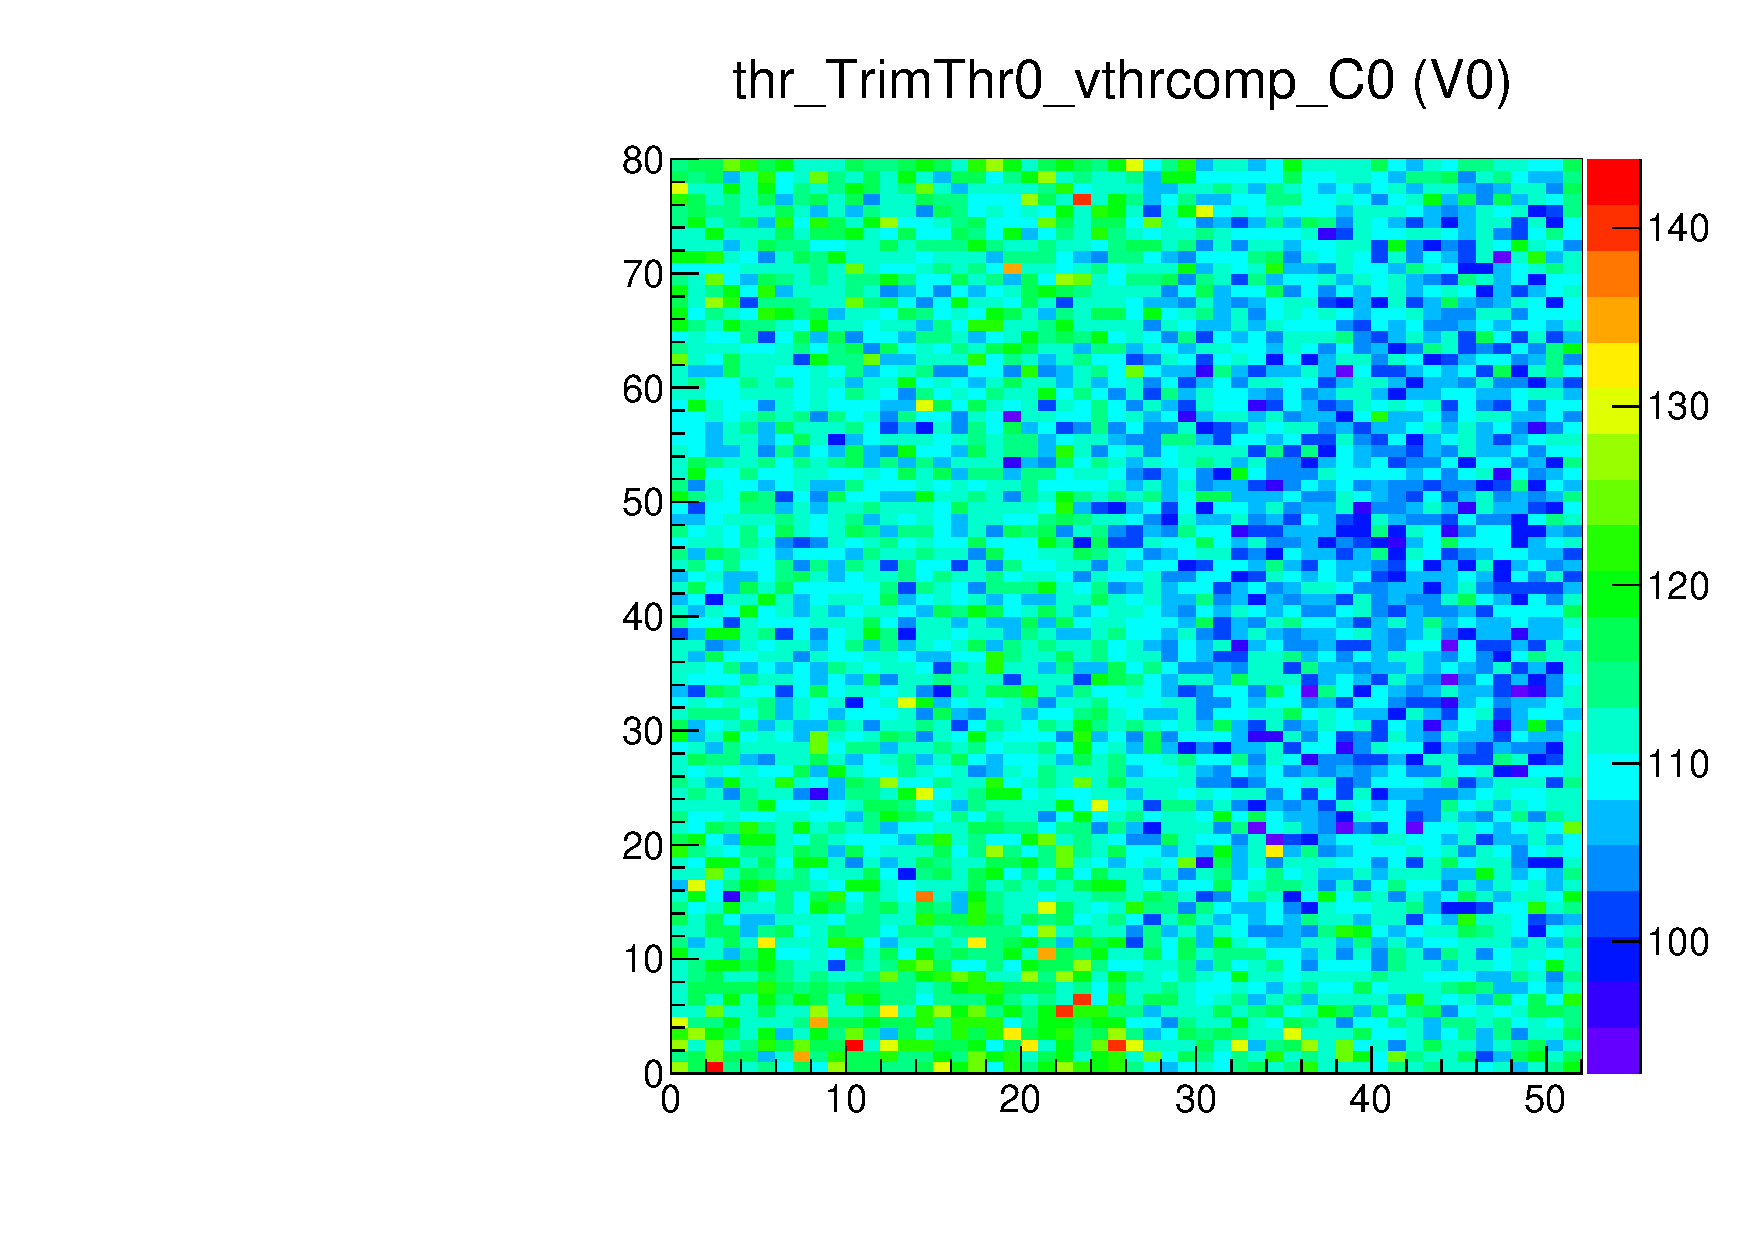
\includegraphics[width=1.0\textwidth]{figures/trim_thr_TrimThr0_vthrcomp.pdf}
  \caption{}
  \label{fig:trim_thr_TrimThr0_vthrcomp}
\end{minipage}
\hspace{0.3cm}
\begin{minipage}{0.45\textwidth}

% from trim test:  scan to get maximal vcal turn-on pixel
  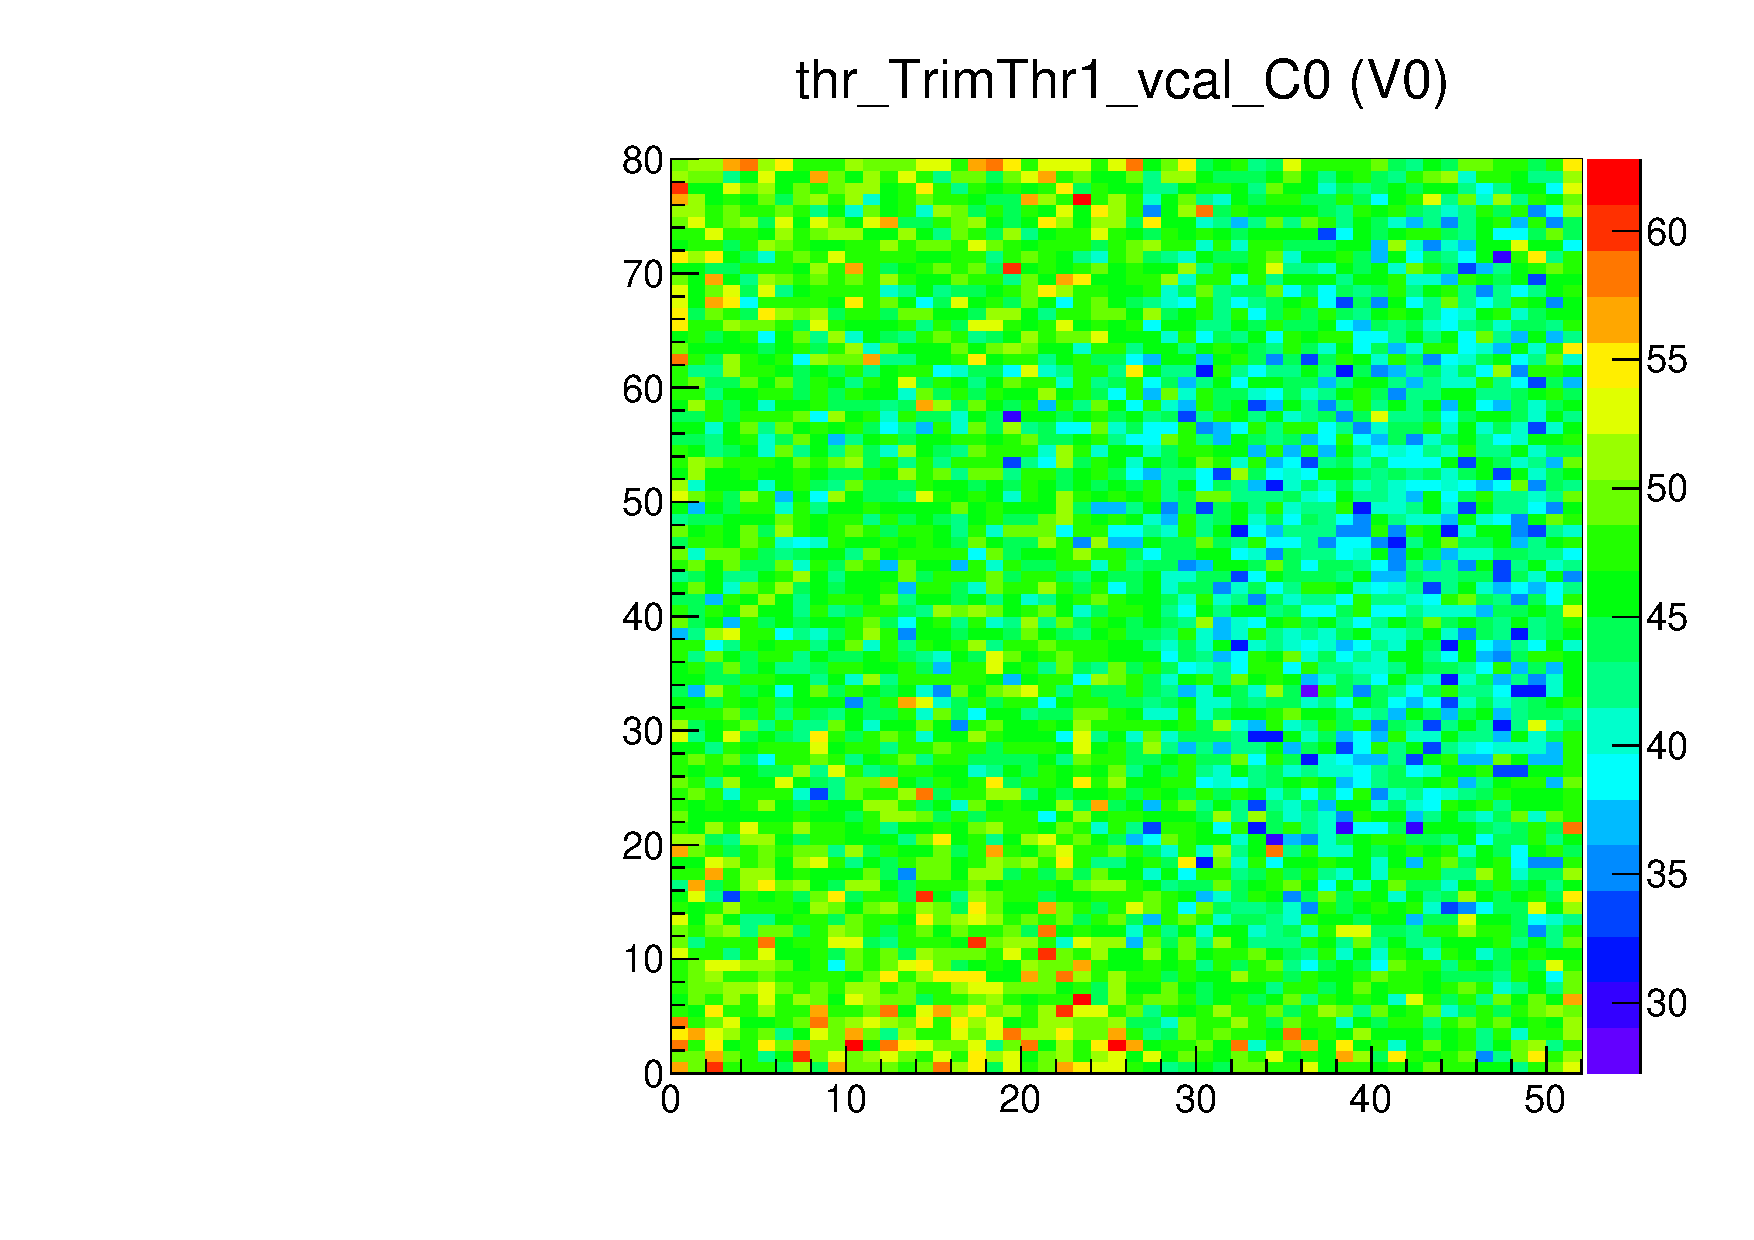
\includegraphics[width=1.0\textwidth]{figures/trim_thr_TrimThr1_vcal.pdf}
  \caption{}
  \label{fig:trim_thr_TrimThr1_vcal}
\end{minipage}
\end{figure}

% from trim test: efficiency in vcal/trim plane, for setting Vtrim

\begin{figure}[!Hp]
\centering
\begin{minipage}{0.45\textwidth}
  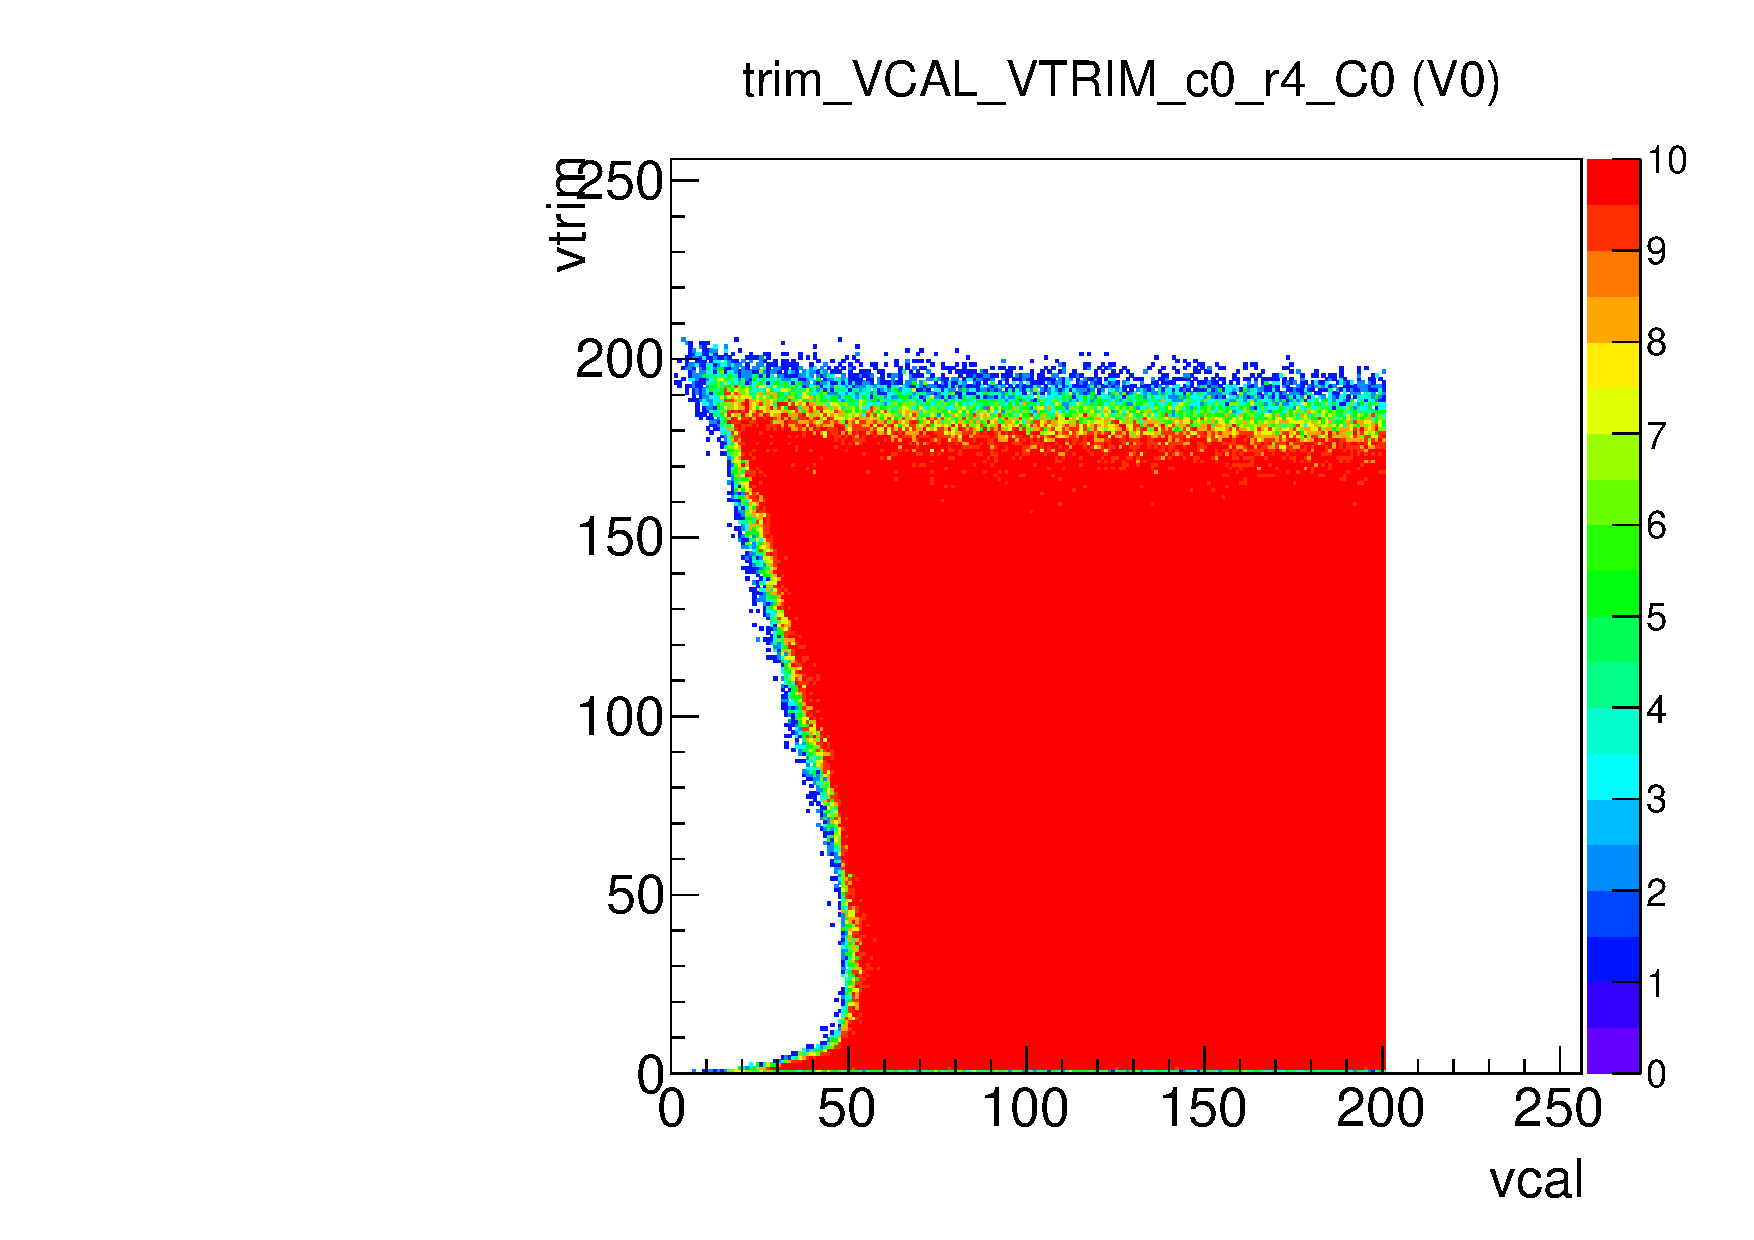
\includegraphics[width=1.0\textwidth]{figures/trim_trim_VCAL_VTRIM.pdf}
  \caption{}
  \label{fig:trim_trim_VCAL_VTRIM}
\end{minipage}
\end{figure}

% from trim test: threshold maps after each iteration of trim correction

\begin{figure}[!Hp]
\centering
\begin{minipage}{0.45\textwidth}
  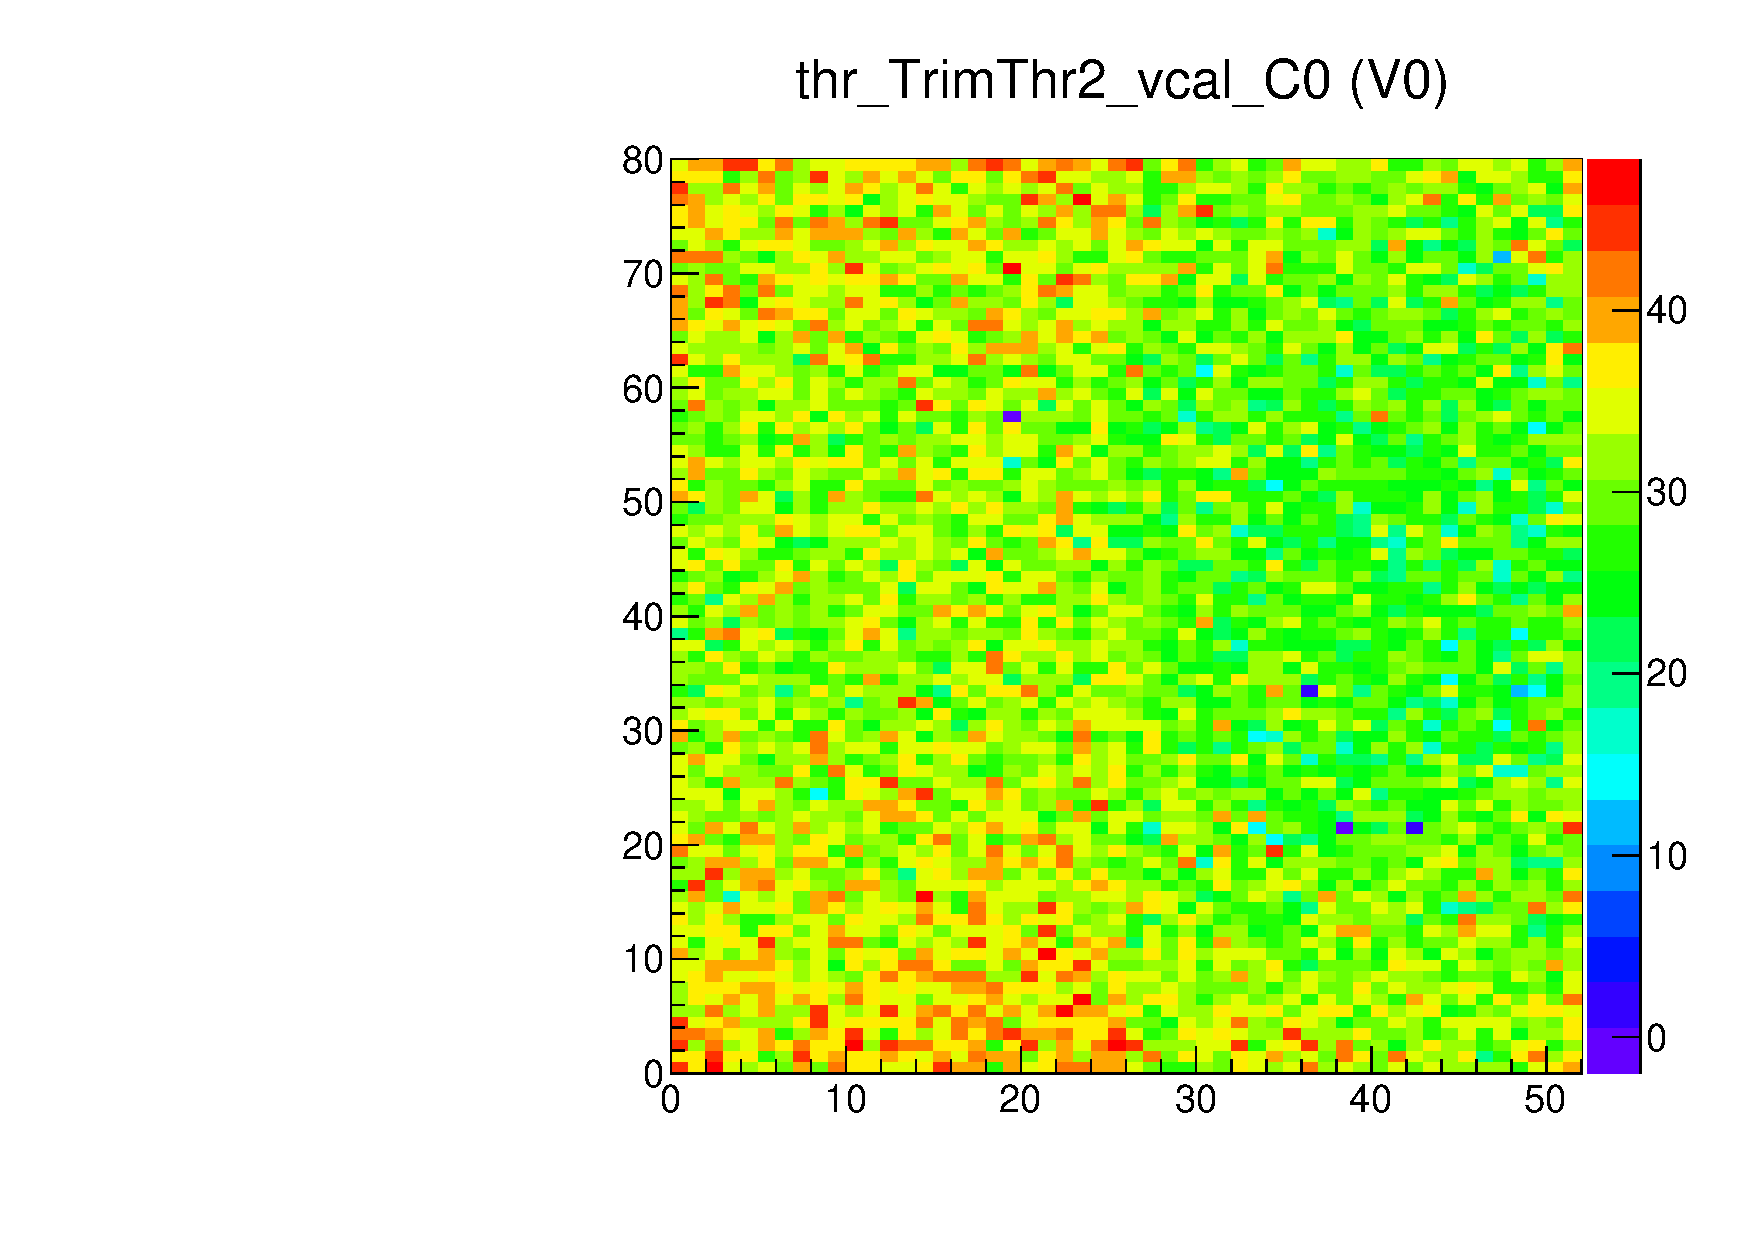
\includegraphics[width=1.0\textwidth]{figures/trim_thr_TrimThr2_vcal.pdf}
  \caption{}
  \label{fig:trim_thr_TrimThr2_vcal}
\end{minipage}
\end{figure}

\begin{figure}[!Hp]
\centering
\begin{minipage}{0.45\textwidth}
  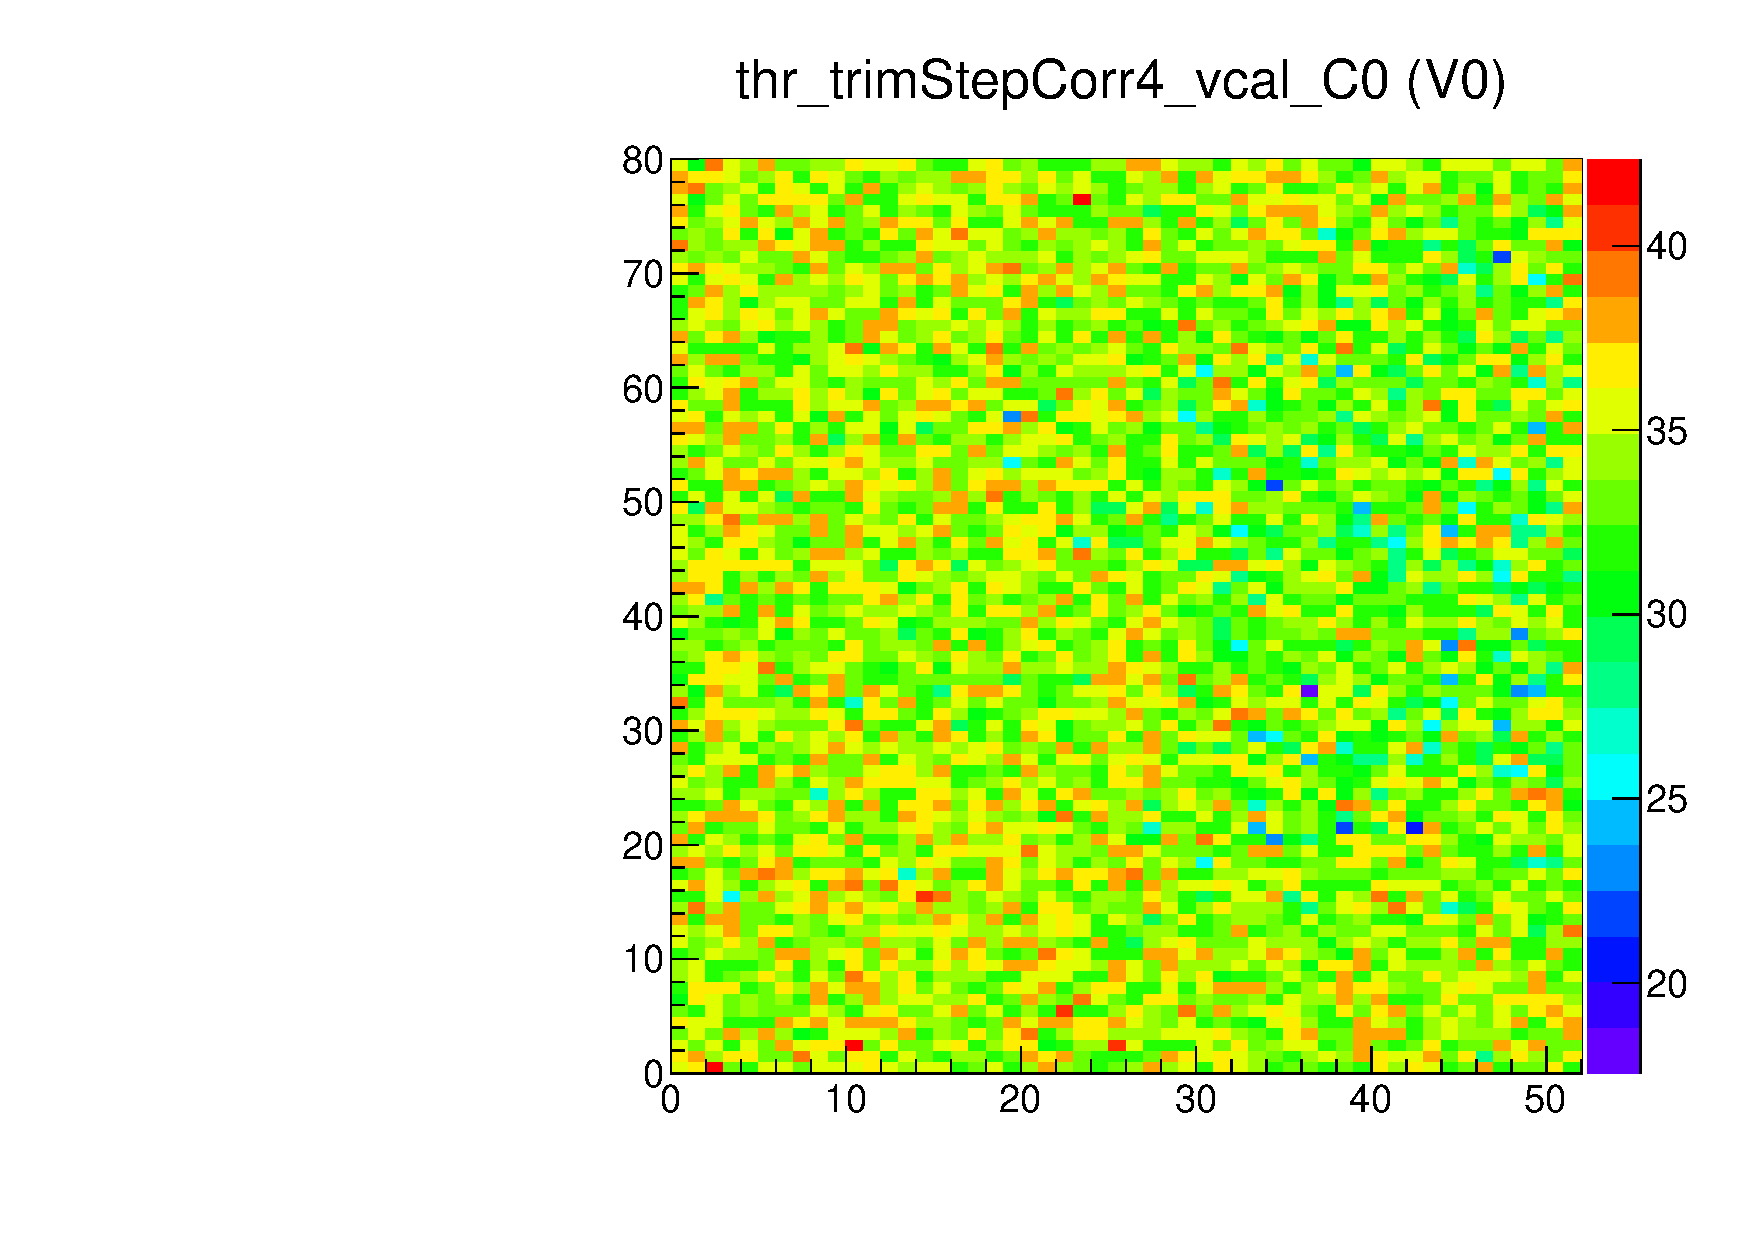
\includegraphics[width=1.0\textwidth]{figures/trim_thr_trimStepCorr4_vcal.pdf}
  \caption{}
  \label{fig:trim_thr_trimStepCorr4_vcal}
\end{minipage}
\hspace{0.3cm}
\begin{minipage}{0.45\textwidth}
  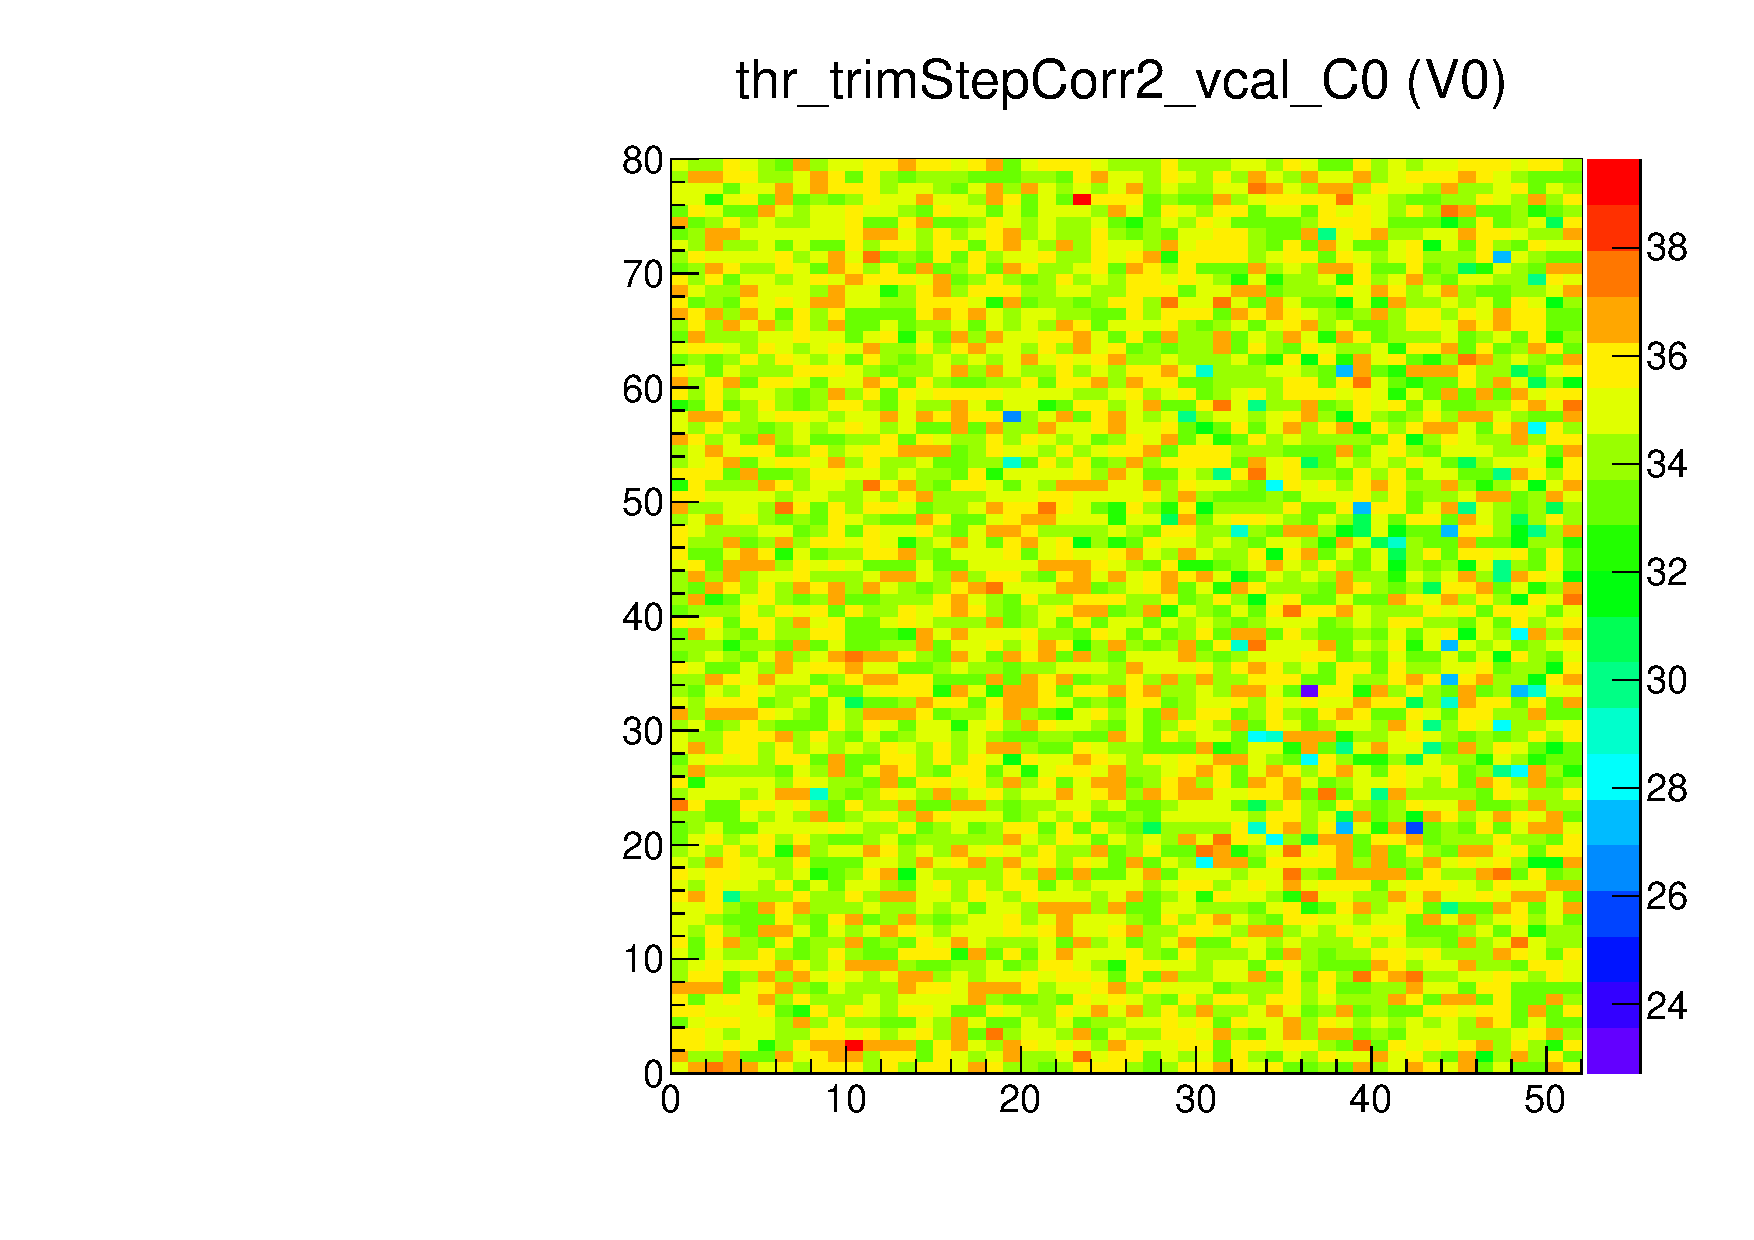
\includegraphics[width=1.0\textwidth]{figures/trim_thr_trimStepCorr2_vcal.pdf}
  \caption{}
  \label{fig:trim_thr_trimStepCorr2_vcal}
\end{minipage}
\end{figure}

\begin{figure}[!Hp]
\centering
\begin{minipage}{0.45\textwidth}
  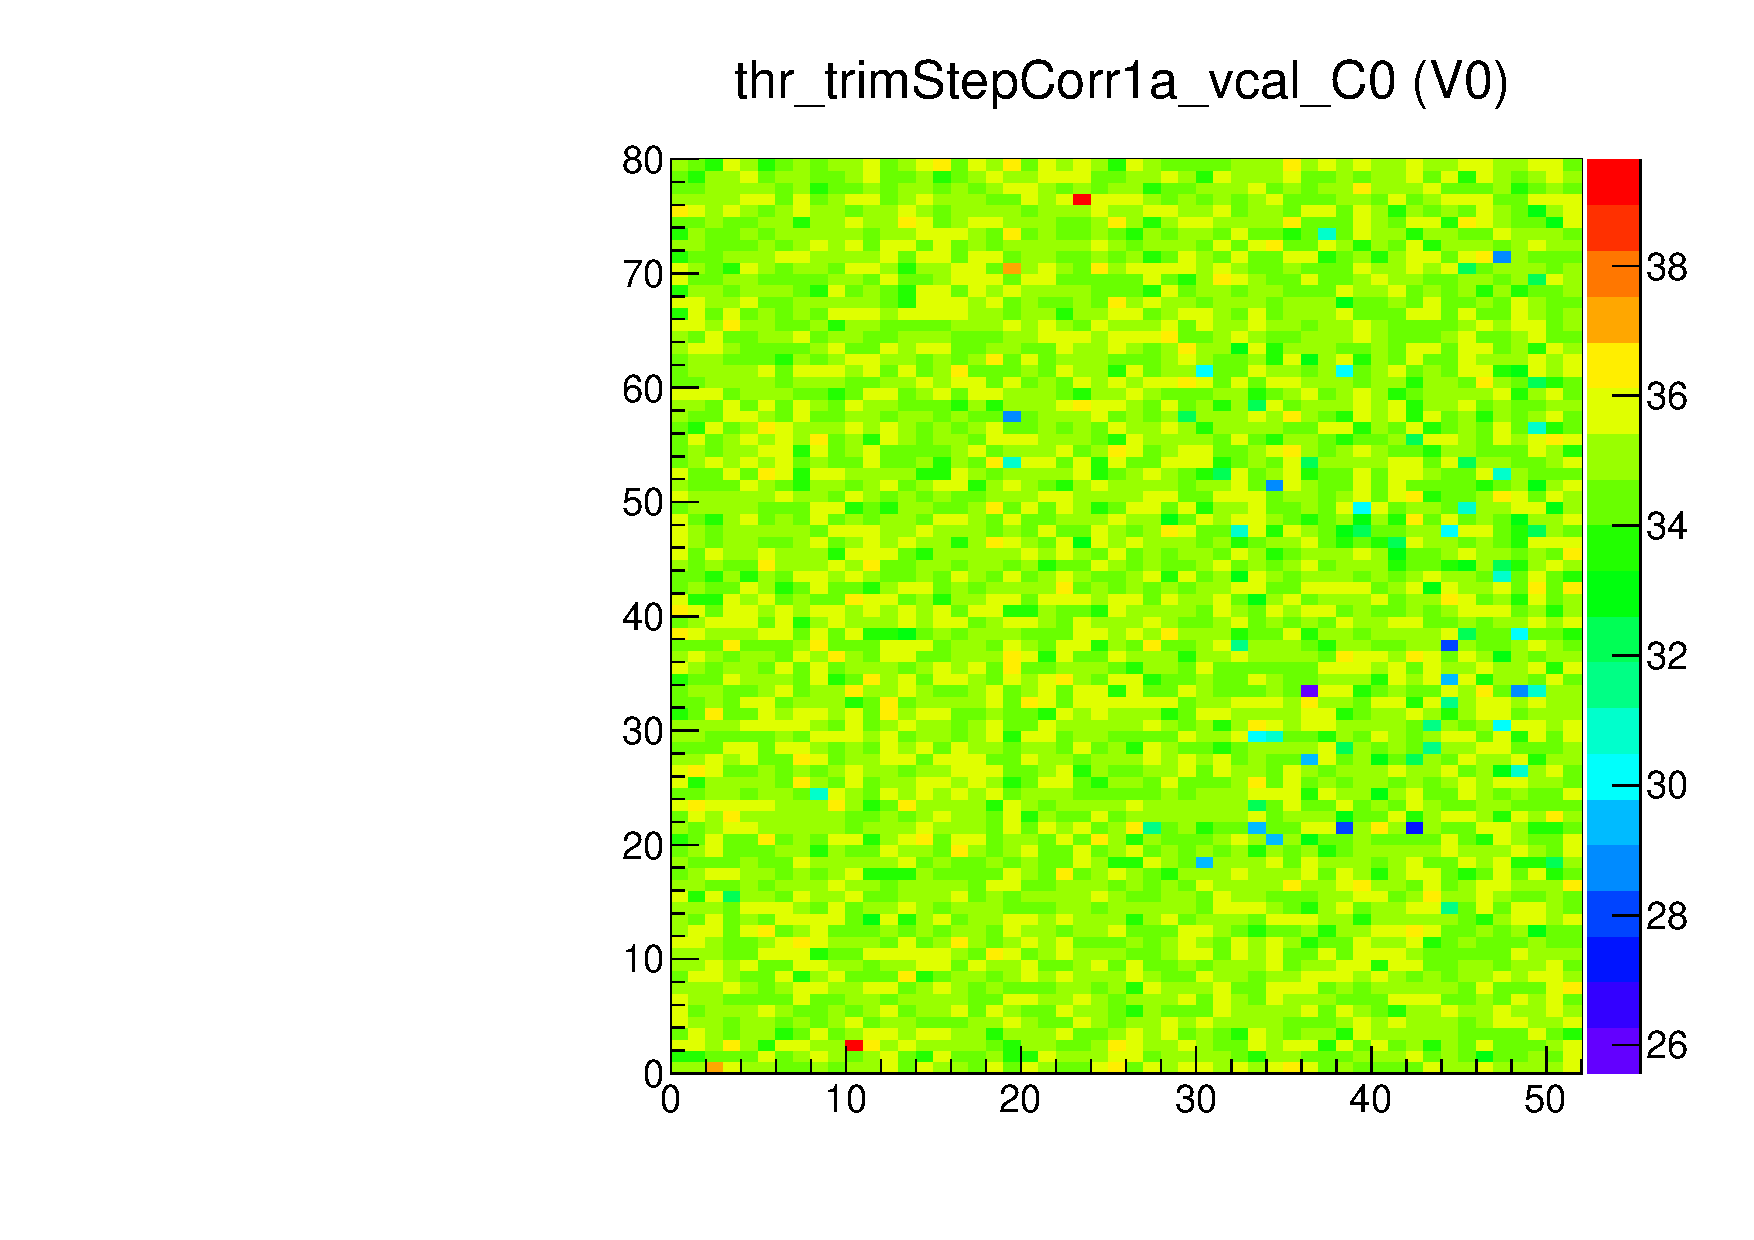
\includegraphics[width=1.0\textwidth]{figures/trim_thr_trimStepCorr1a_vcal.pdf}
  \caption{}
  \label{fig:trim_thr_trimStepCorr1a_vcal}
\end{minipage}
\hspace{0.3cm}
\begin{minipage}{0.45\textwidth}
  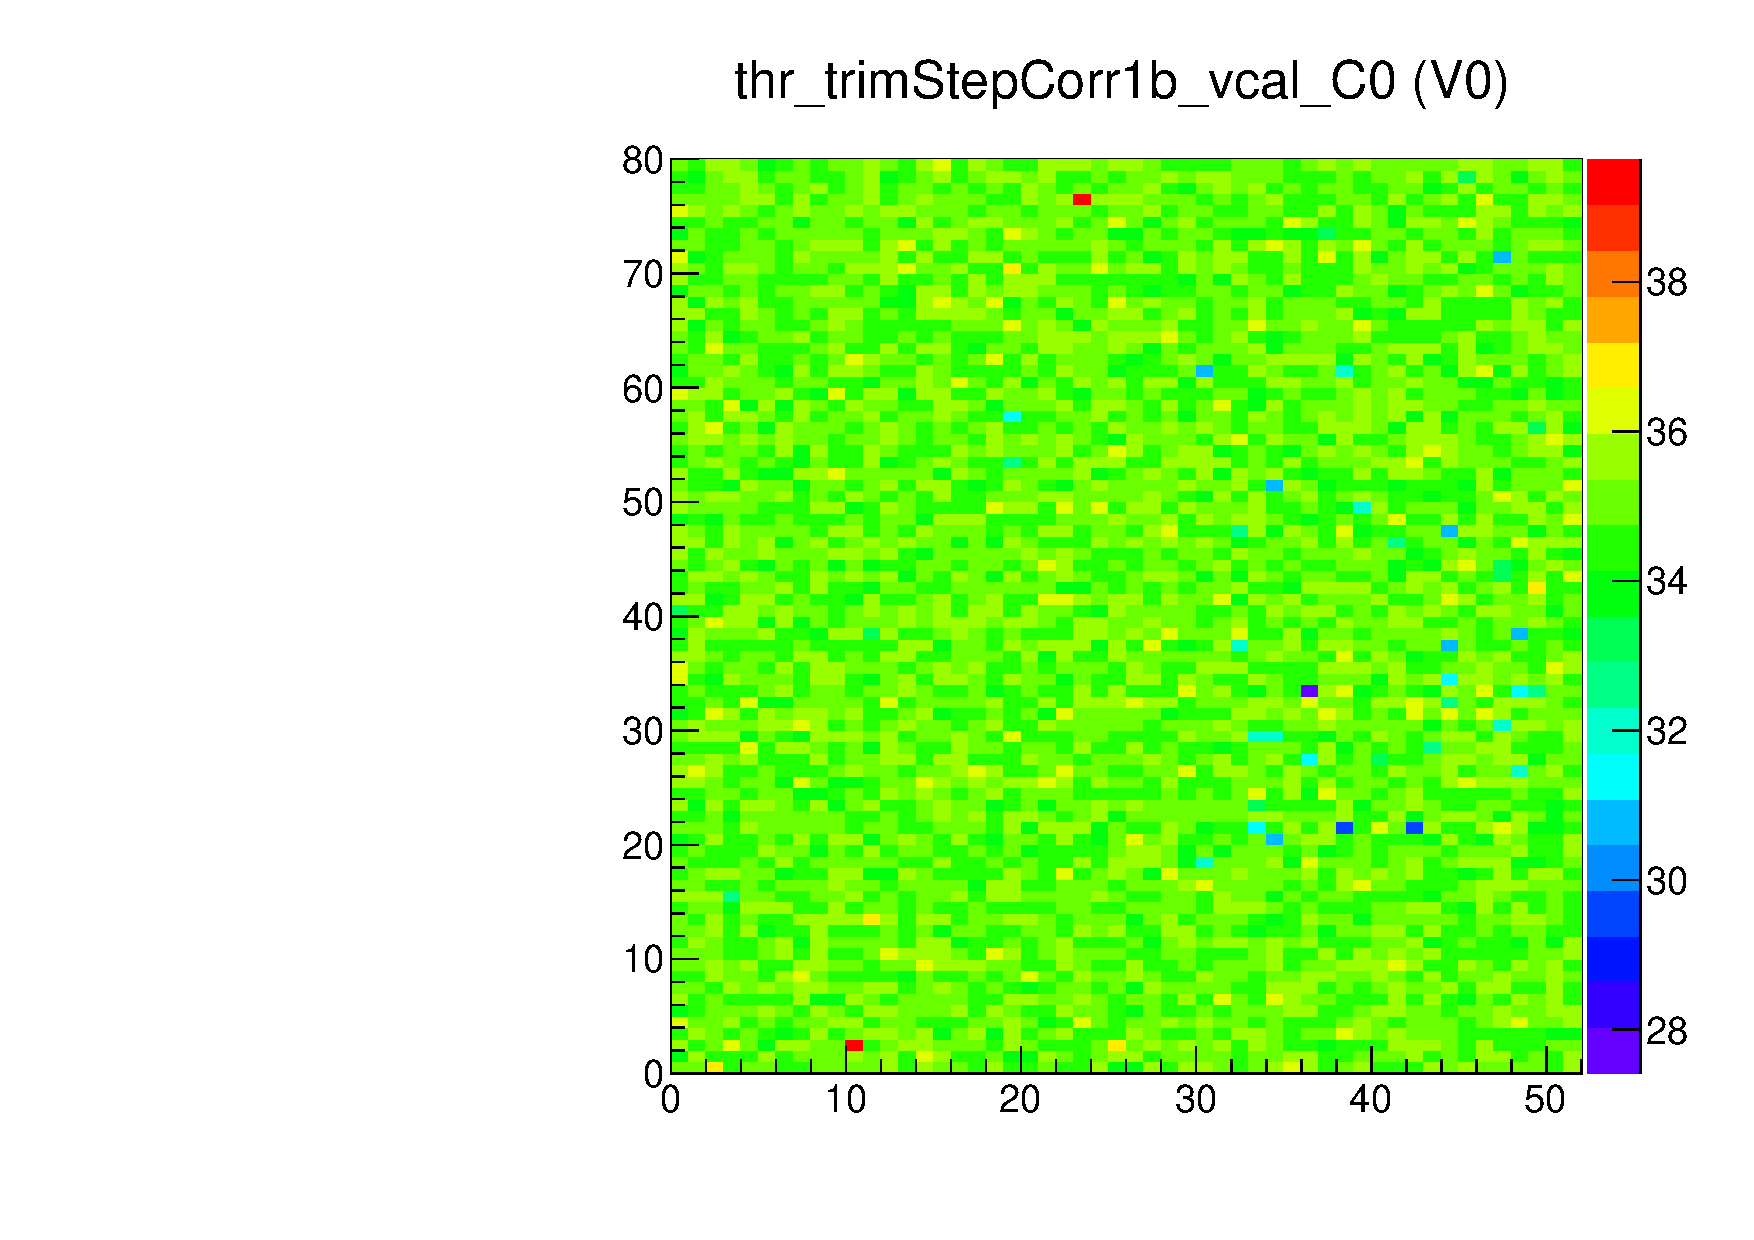
\includegraphics[width=1.0\textwidth]{figures/trim_thr_trimStepCorr1b_vcal.pdf}
  \caption{}
  \label{fig:trim_thr_trimStepCorr1b_vcal}
\end{minipage}
\end{figure}


% from trim test:  optimized trim bits

\begin{figure}[!Hp]
\centering
\begin{minipage}{0.45\textwidth}
  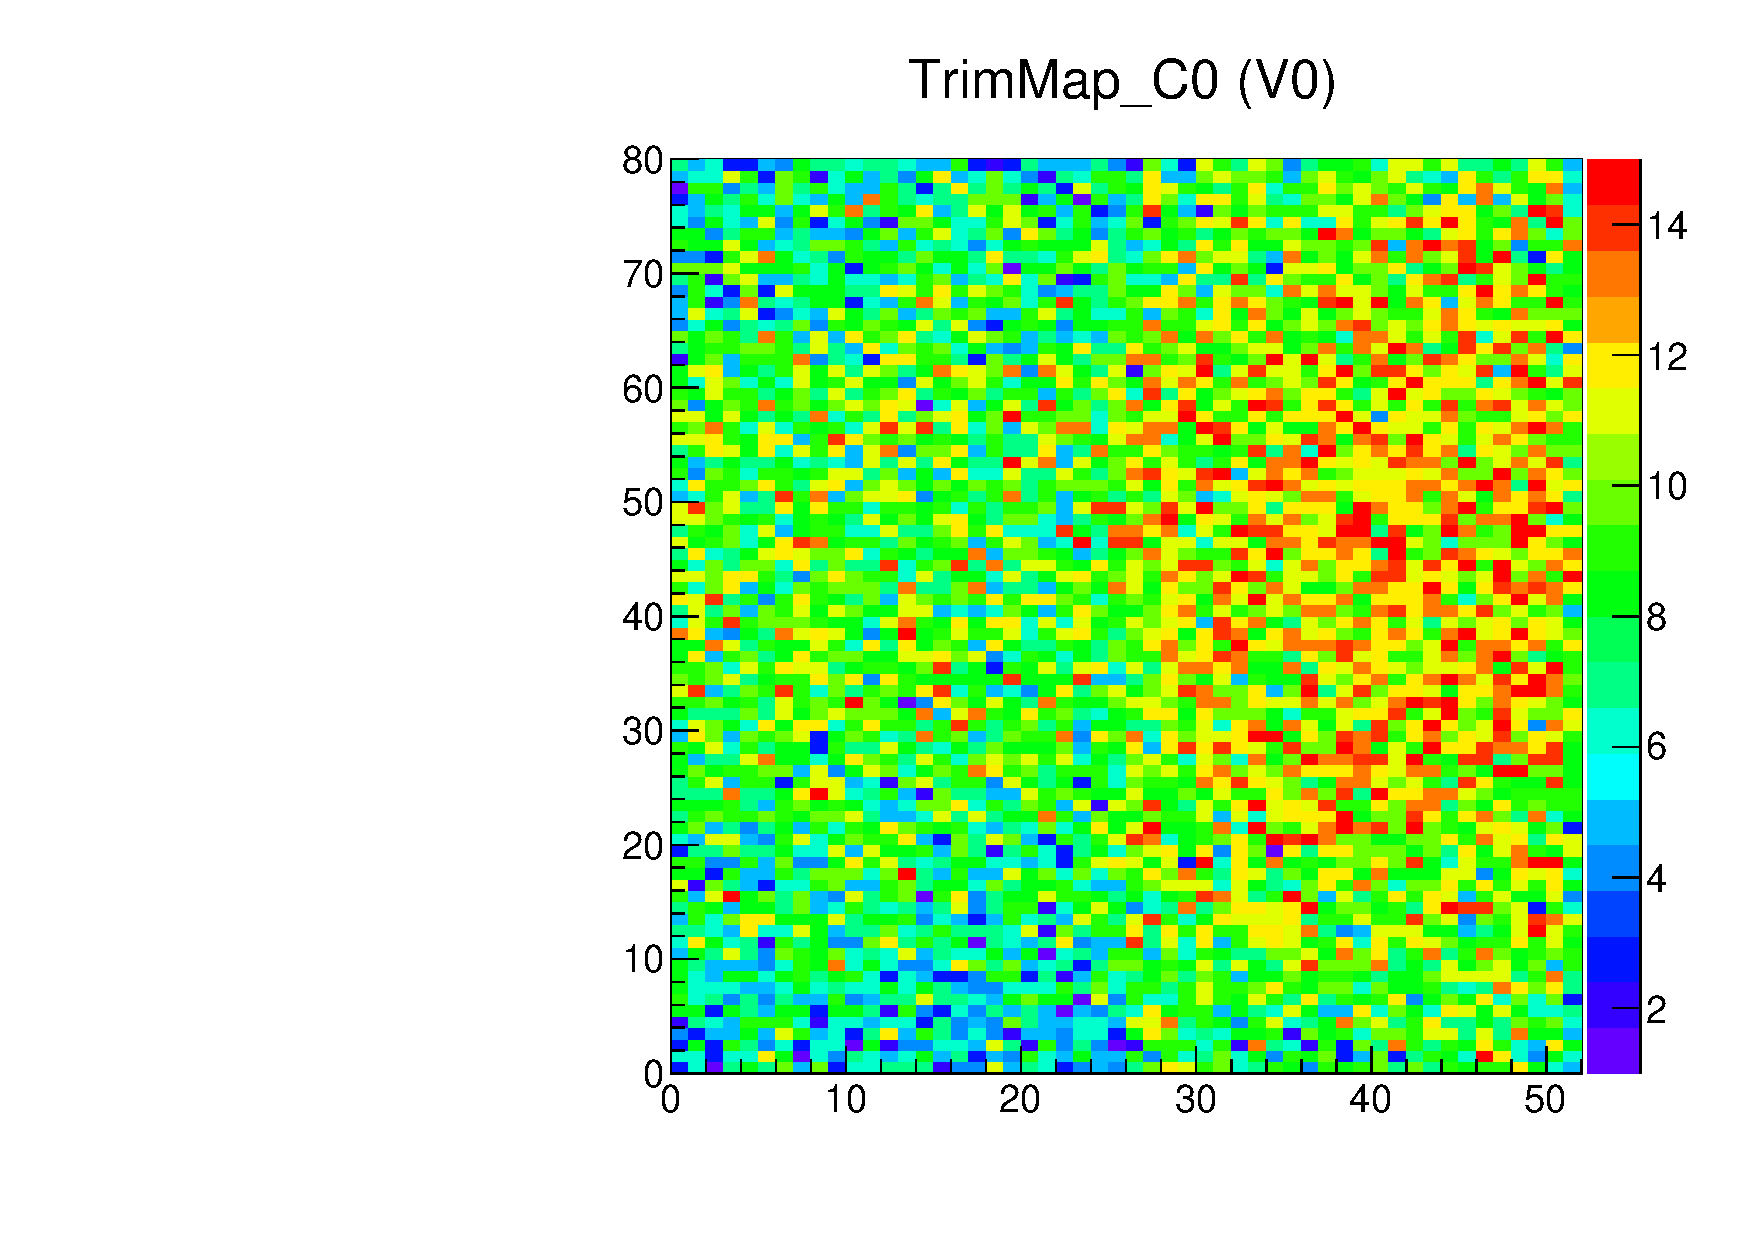
\includegraphics[width=1.0\textwidth]{figures/trim_TrimMap.pdf}
  \caption{\roc map of the optimized trim bit values (0-15).}
  \label{fig:trim_TrimMap}
\end{minipage}
\hspace{0.3cm}
\begin{minipage}{0.45\textwidth}
  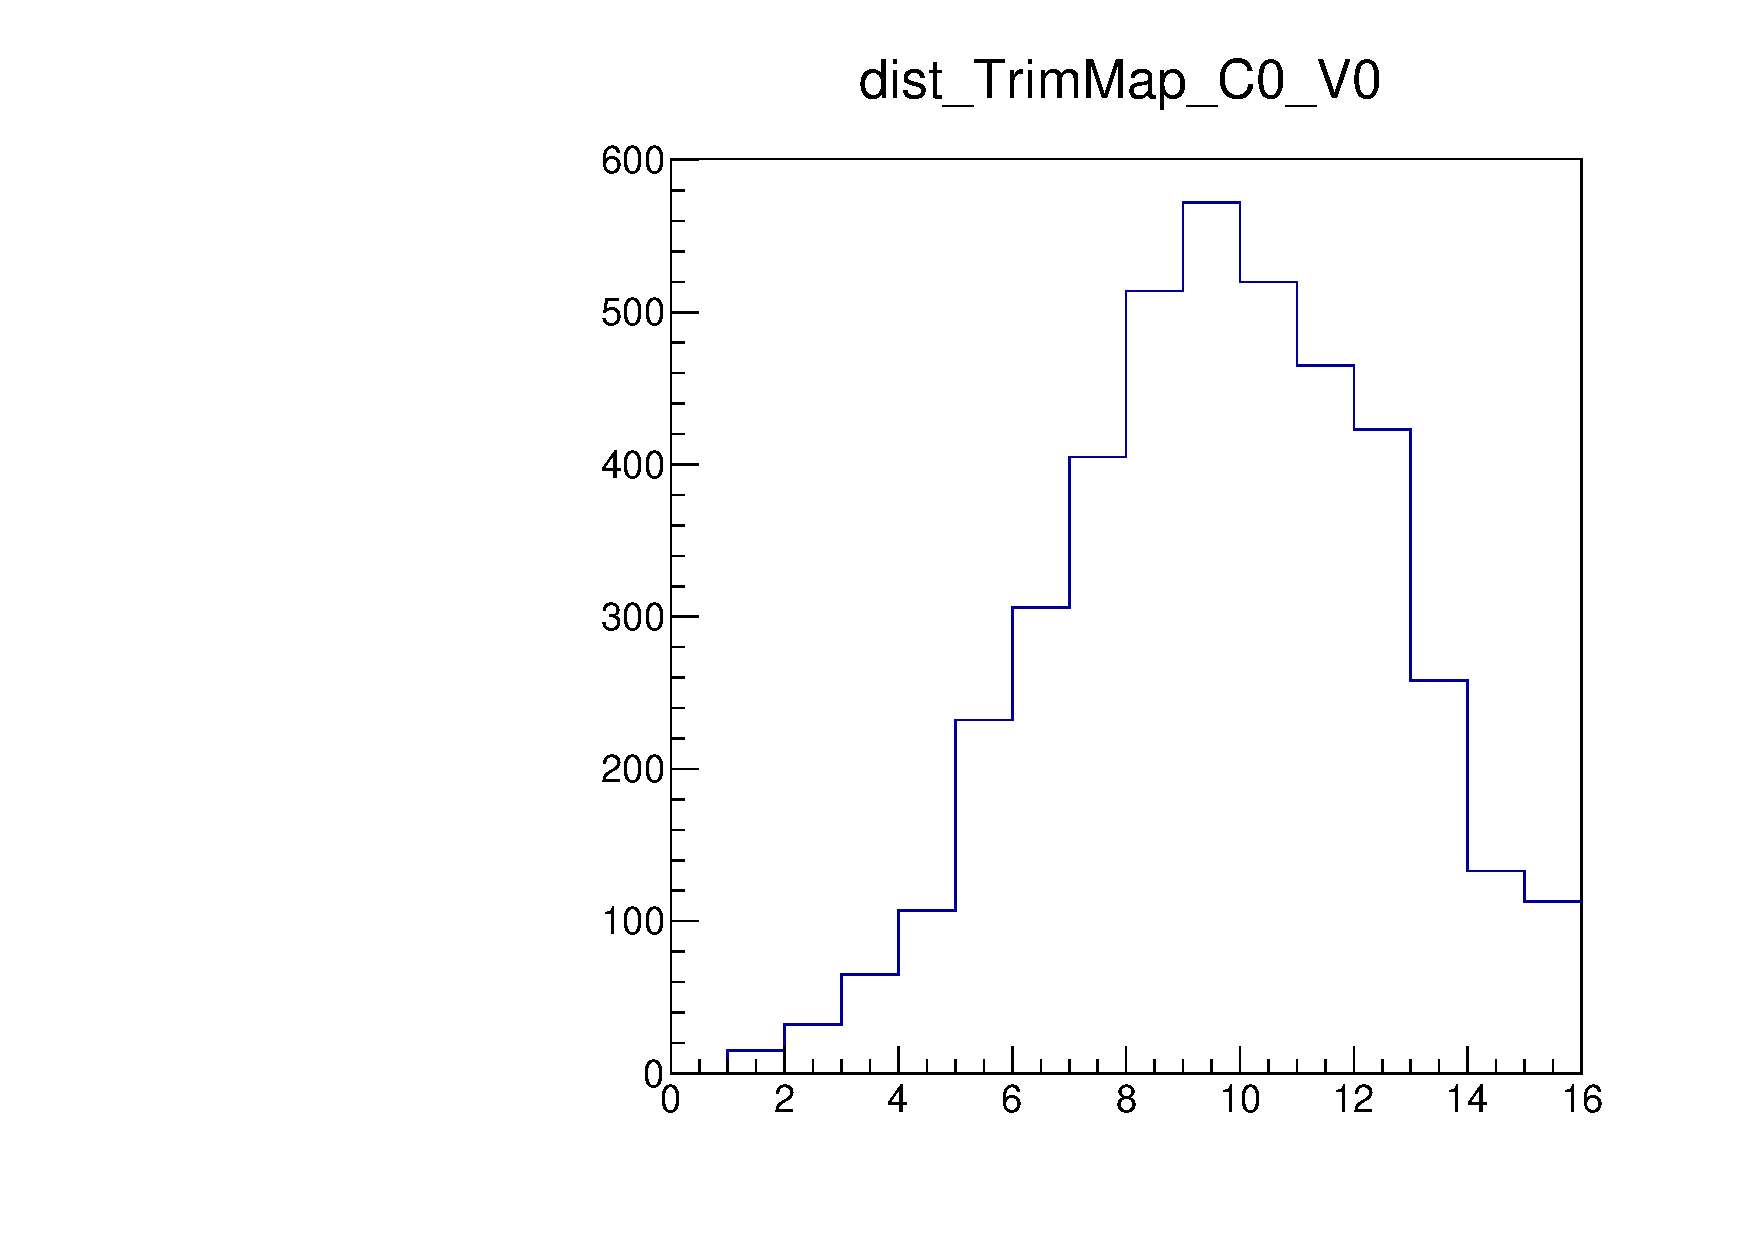
\includegraphics[width=1.0\textwidth]{figures/trim_dist_TrimMap.pdf}
  \caption{1D distribution of the optimized trim bit values (0-15).}
  \label{fig:trim_dist_TrimMap}
\end{minipage}
\end{figure}

% from trim test: vcal turn-on after trimming

\begin{figure}[!Hp]
\centering
\begin{minipage}{0.45\textwidth}
  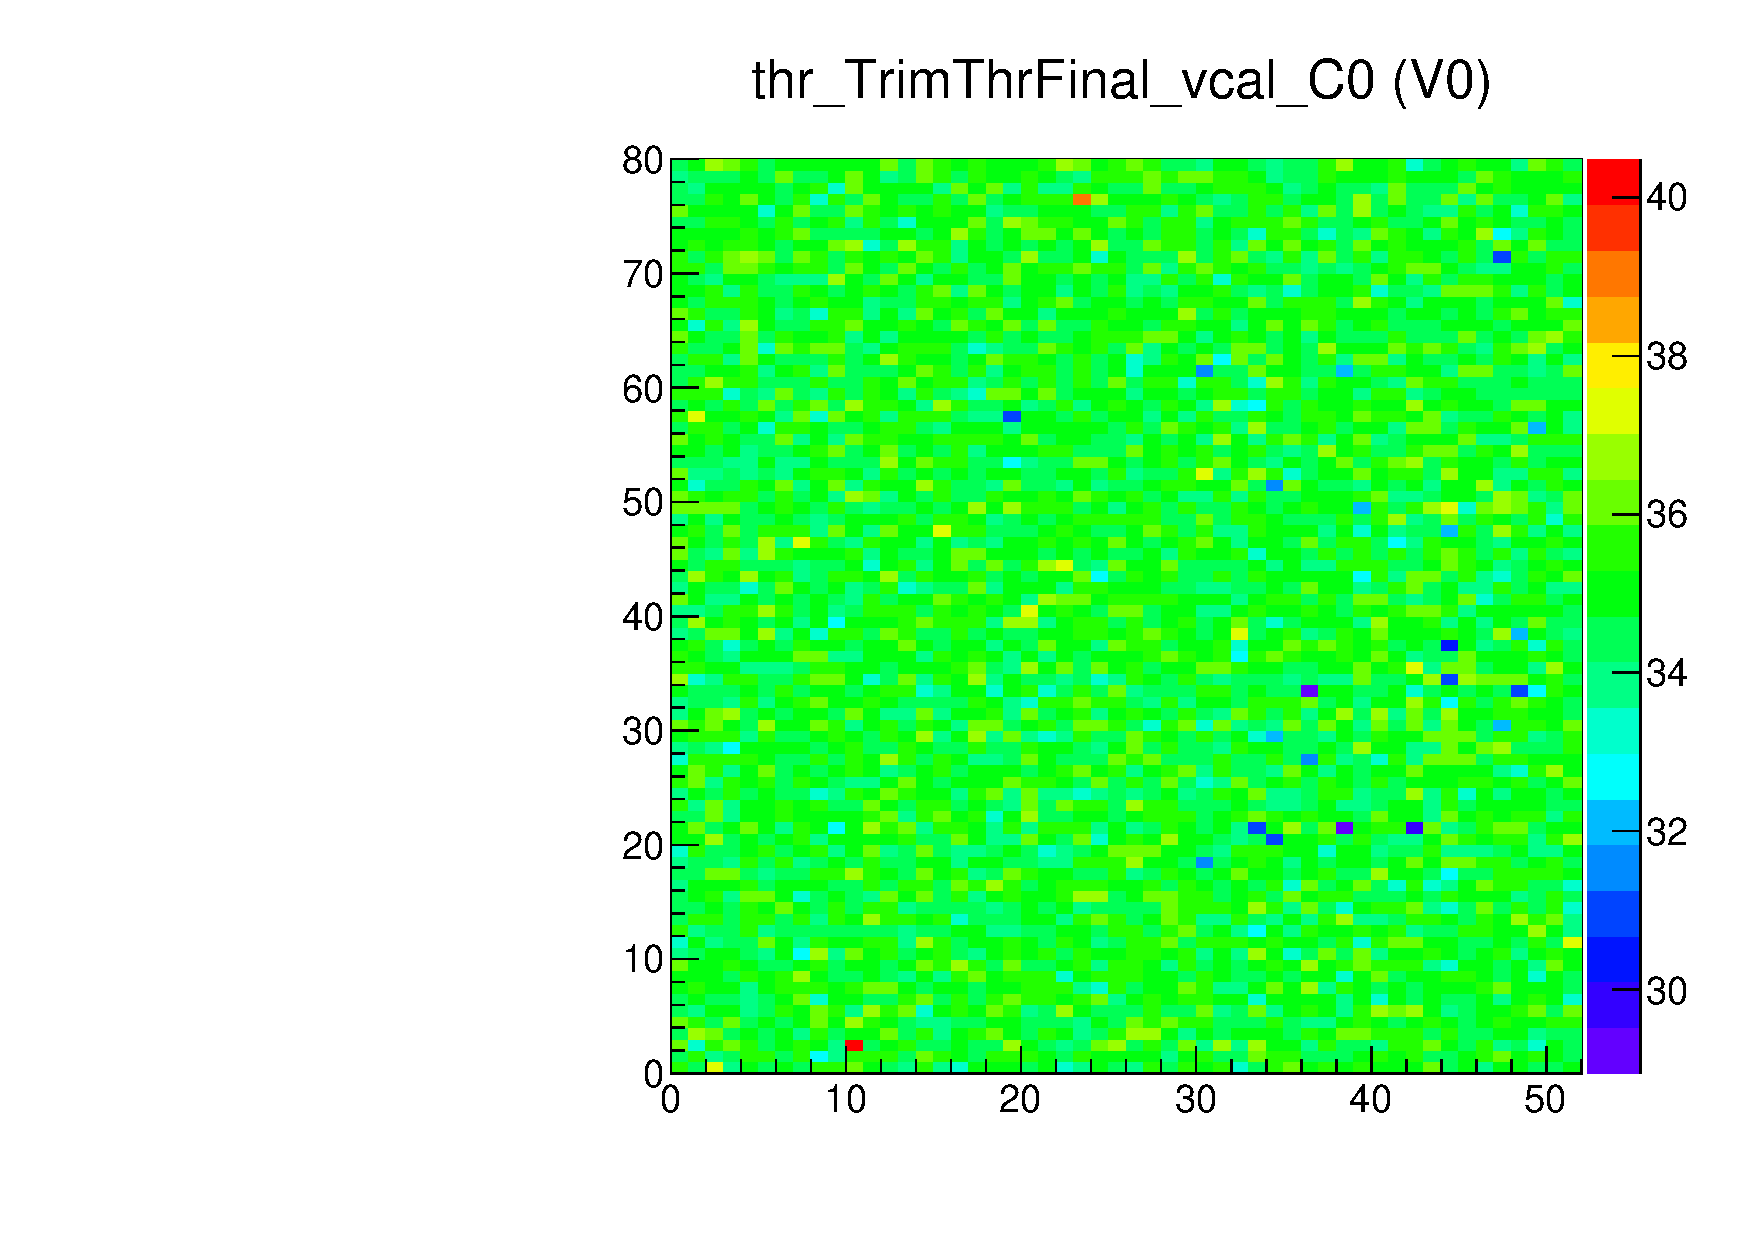
\includegraphics[width=1.0\textwidth]{figures/trim_thr_TrimThrFinal_vcal.pdf}
  \caption{\roc map of the \vcal turn-on thresholds with optimized trim parameters.}
  \label{fig:trim_thr_TrimThrFinal_vcal}
\end{minipage}
\hspace{0.3cm}
\begin{minipage}{0.45\textwidth}
  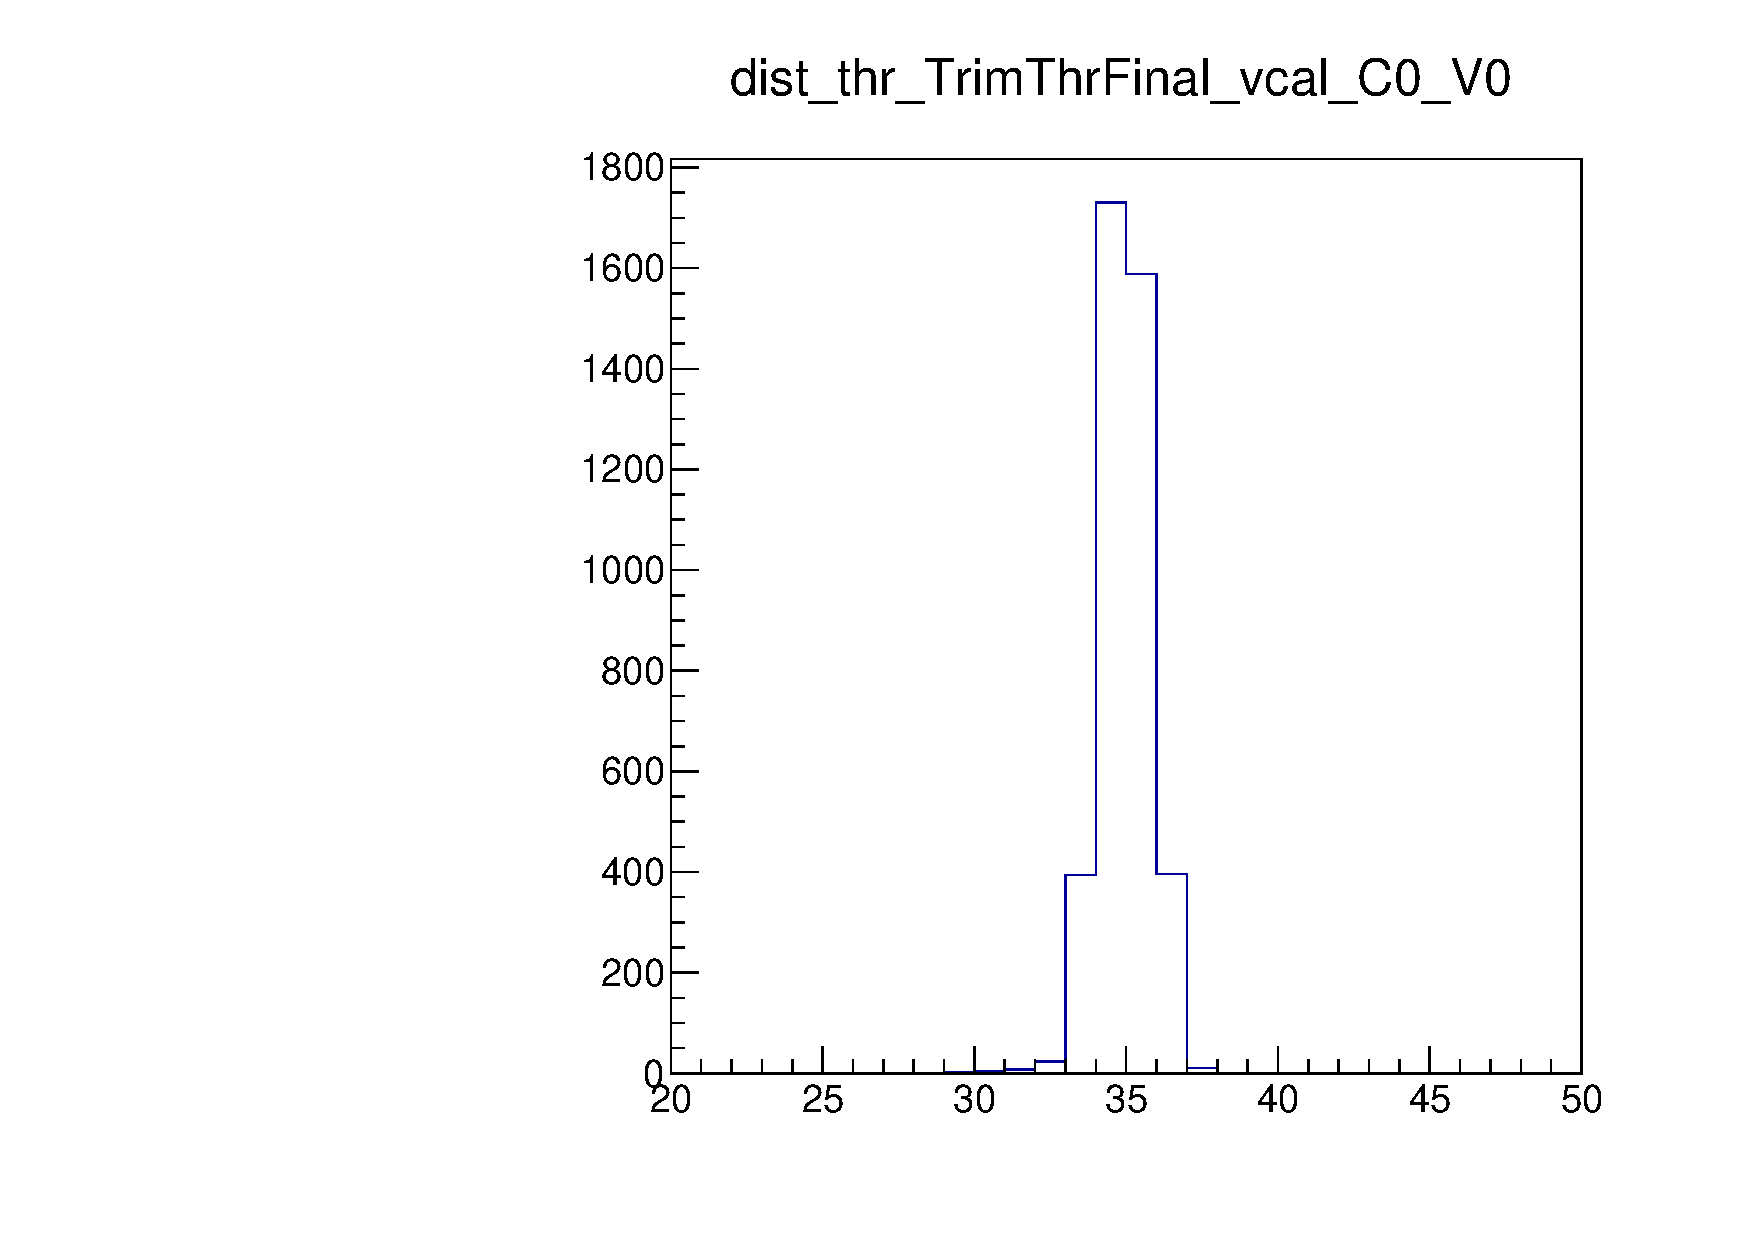
\includegraphics[width=1.0\textwidth]{figures/trim_dist_thr_TrimThrFinal_vcal.pdf}
  \caption{1D distribution of the \vcal turn-on thresholds with optimized trim parameters. [original range 0-255]}
  \label{fig:trim_dist_thr_TrimThrFinal_vcal}
\end{minipage}
\end{figure}


% ---------------------------------------------------------------------


% from trim bit test: untrimmed thresholds (trim bits = 15)

\begin{figure}[!Hp]
\centering
\begin{minipage}{0.45\textwidth}
  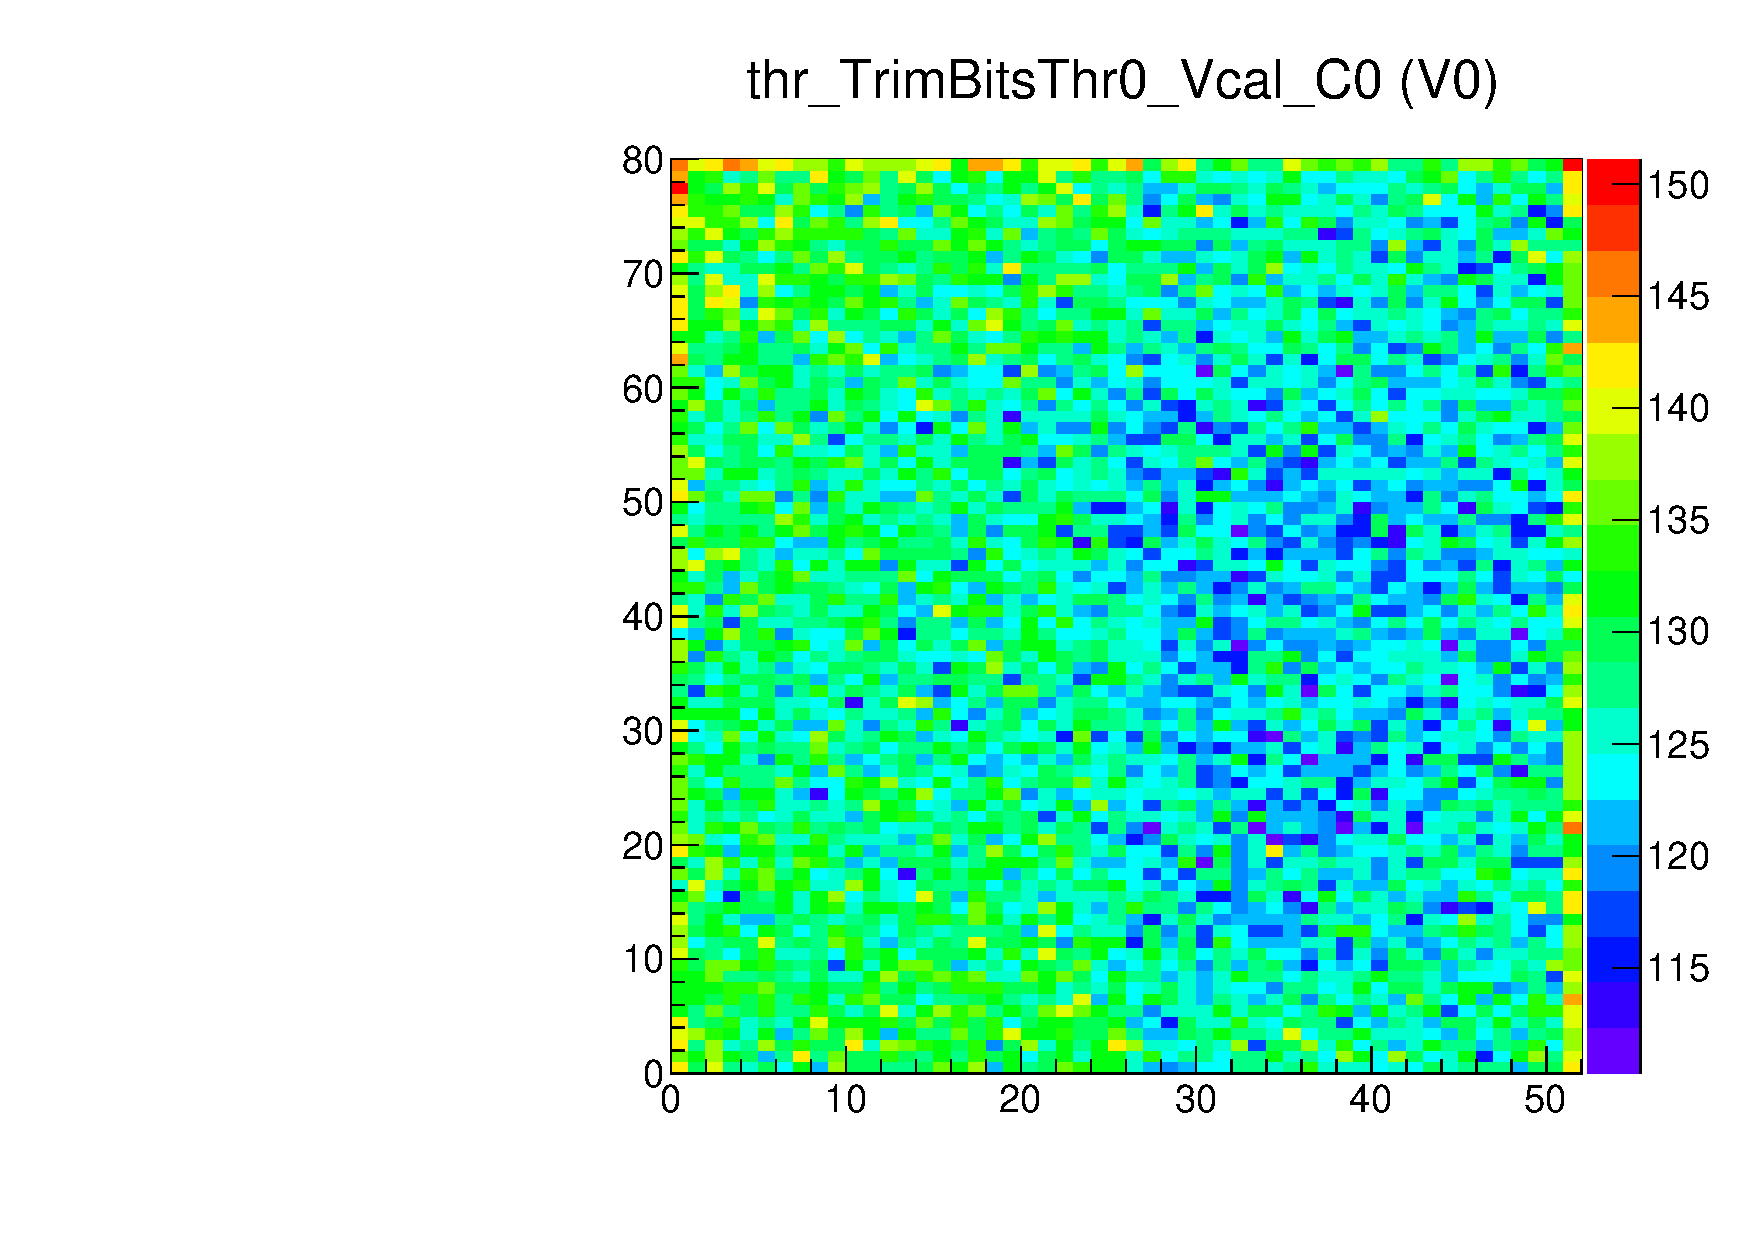
\includegraphics[width=1.0\textwidth]{figures/trim_thr_TrimBitsThr0_Vcal.pdf}
  \caption{}
  \label{fig:trim_thr_TrimBitsThr0_Vcal}
\end{minipage}
\end{figure}


% from trim bits test:  vcal thresholds for different trim bit values trim_thr_TrimThr

\begin{figure}[!Hp]
\centering
\begin{minipage}{0.45\textwidth}
  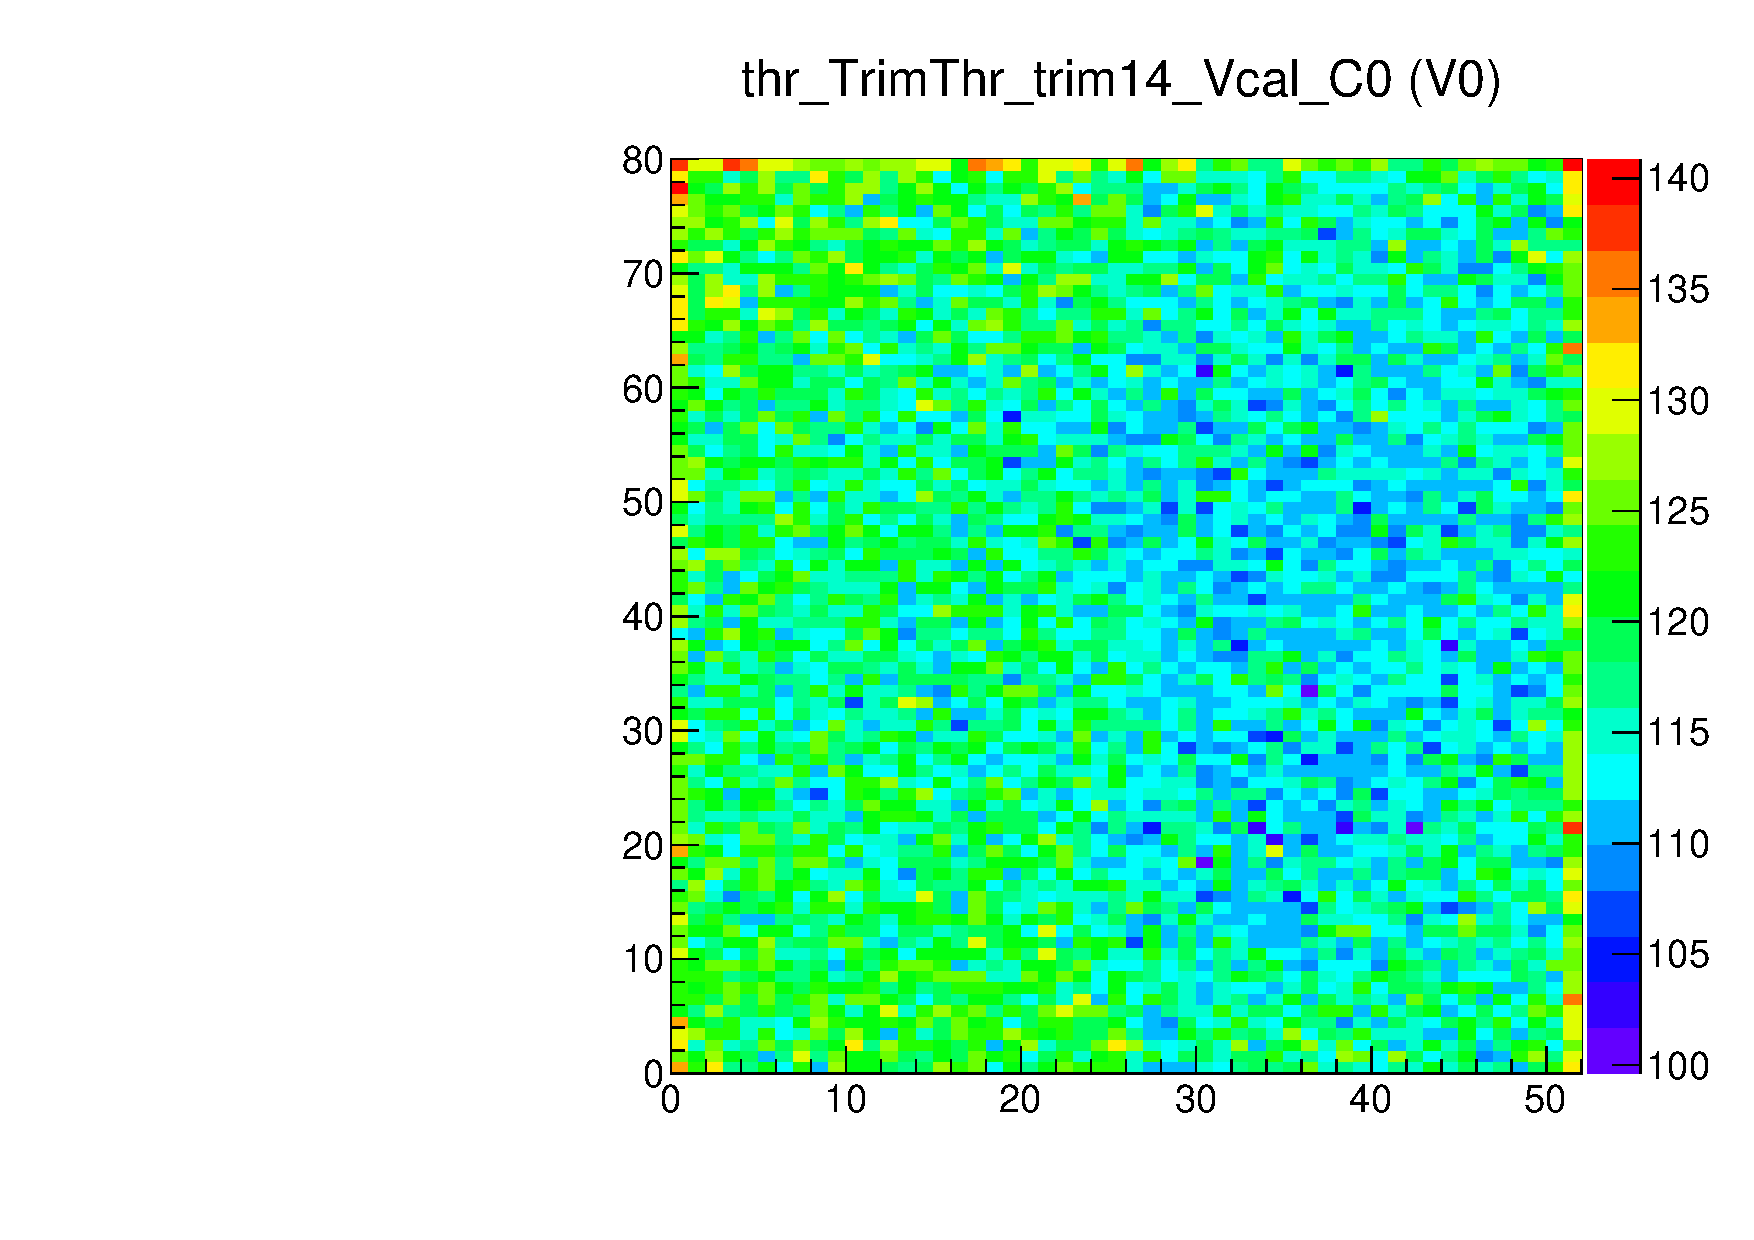
\includegraphics[width=1.0\textwidth]{figures/trim_thr_TrimThr_trim14_Vcal.pdf}
  \caption{}
  \label{fig:trim_thr_TrimThr_trim14_Vcal}
\end{minipage}
\hspace{0.3cm}
\begin{minipage}{0.45\textwidth}
  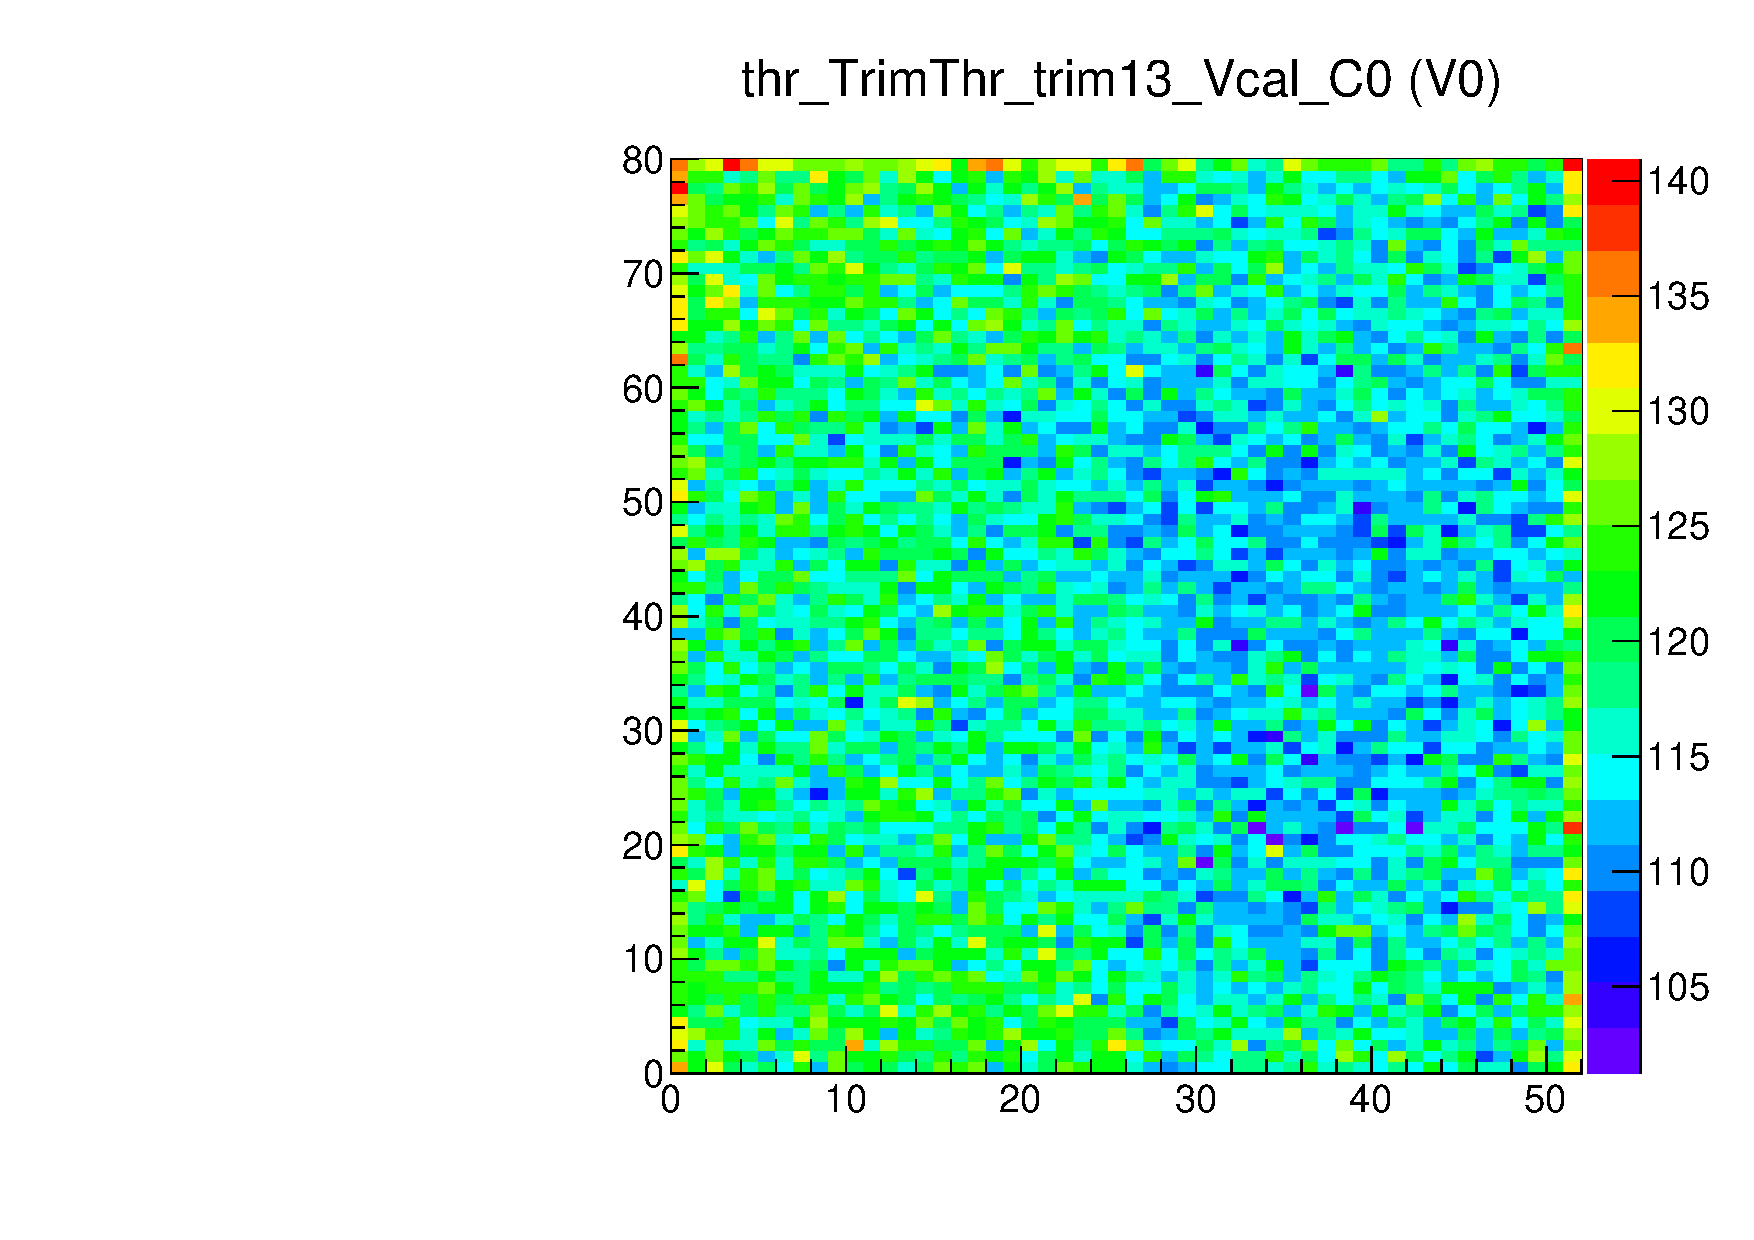
\includegraphics[width=1.0\textwidth]{figures/trim_thr_TrimThr_trim13_Vcal.pdf}
  \caption{}
  \label{fig:trim_thr_TrimThr_trim13_Vcal}
\end{minipage}
\end{figure}

\begin{figure}[!Hp]
\centering
\begin{minipage}{0.45\textwidth}
  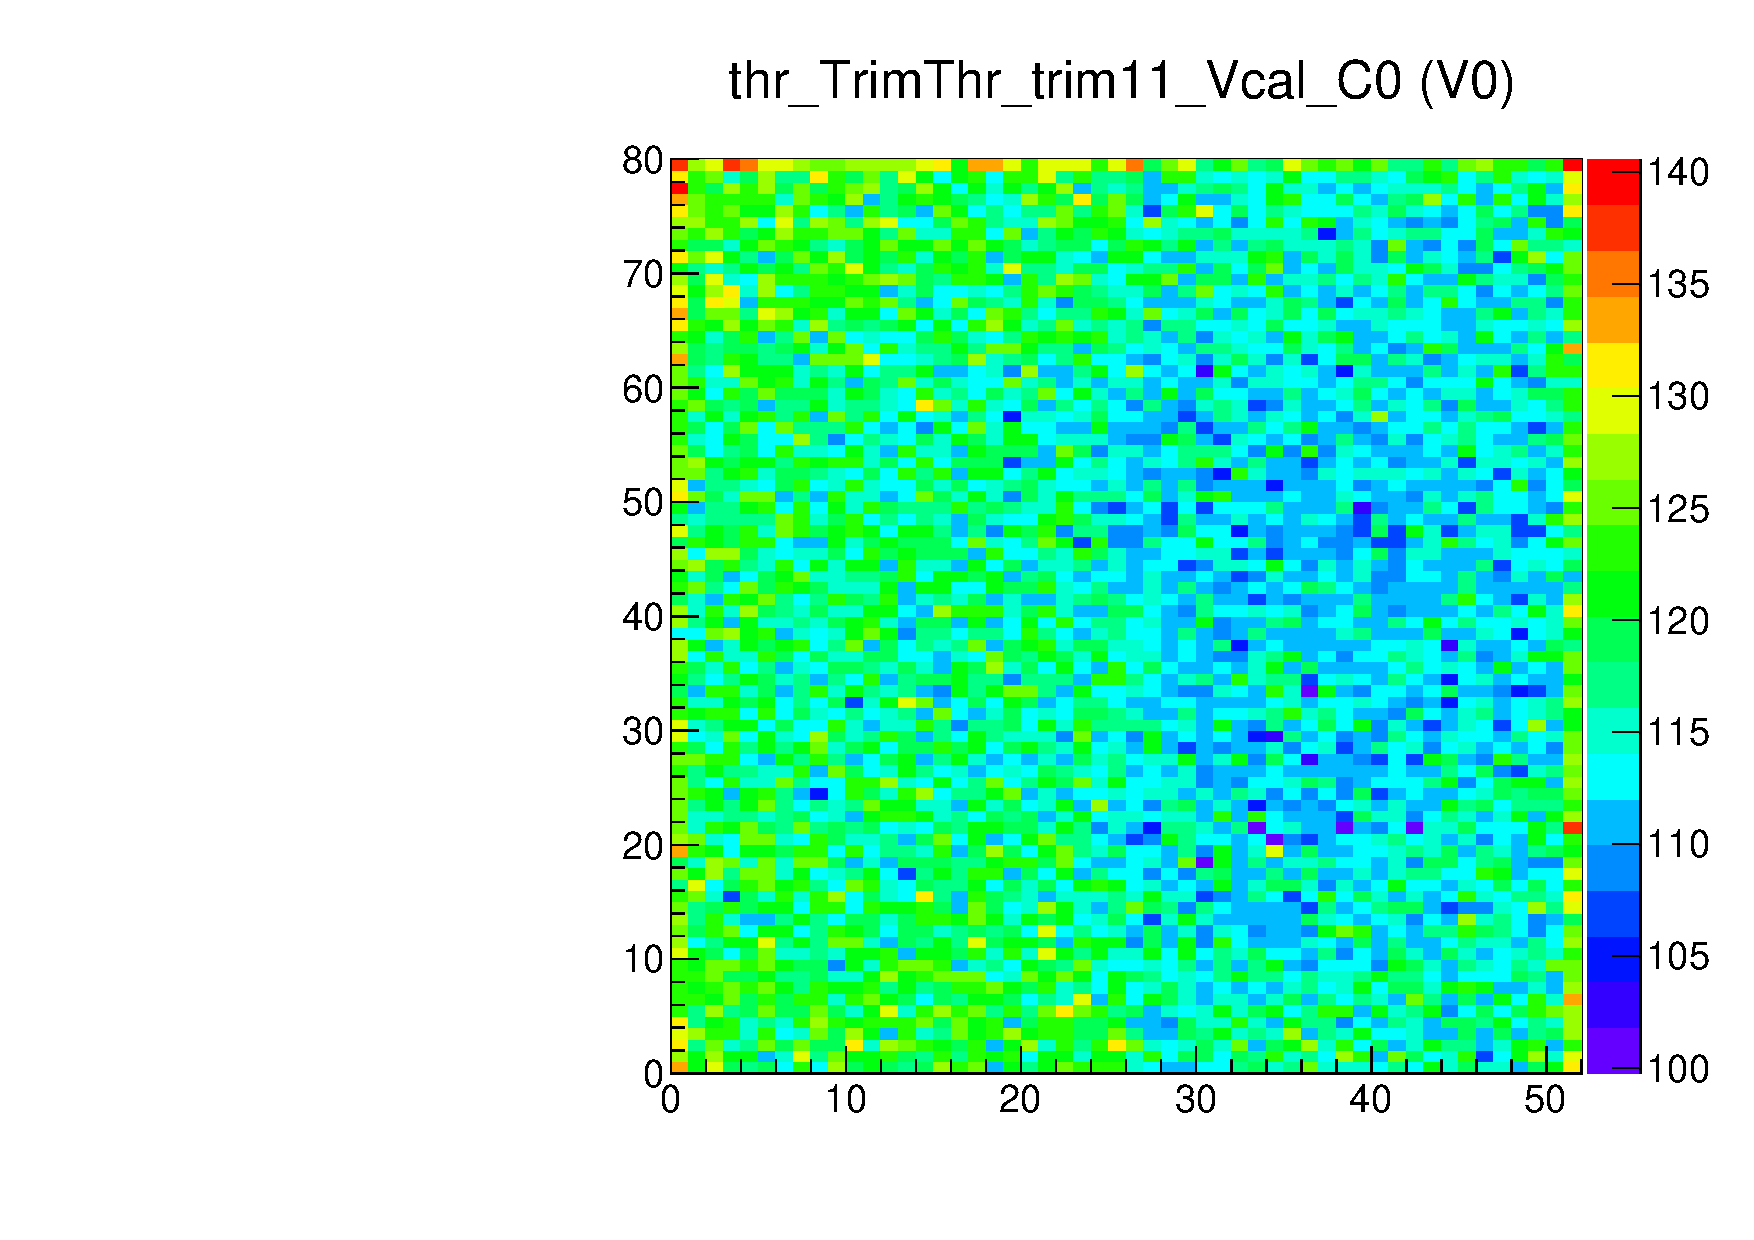
\includegraphics[width=1.0\textwidth]{figures/trim_thr_TrimThr_trim11_Vcal.pdf}
  \caption{}
  \label{fig:trim_thr_TrimThr_trim11_Vcal}
\end{minipage}
\hspace{0.3cm}
\begin{minipage}{0.45\textwidth}
  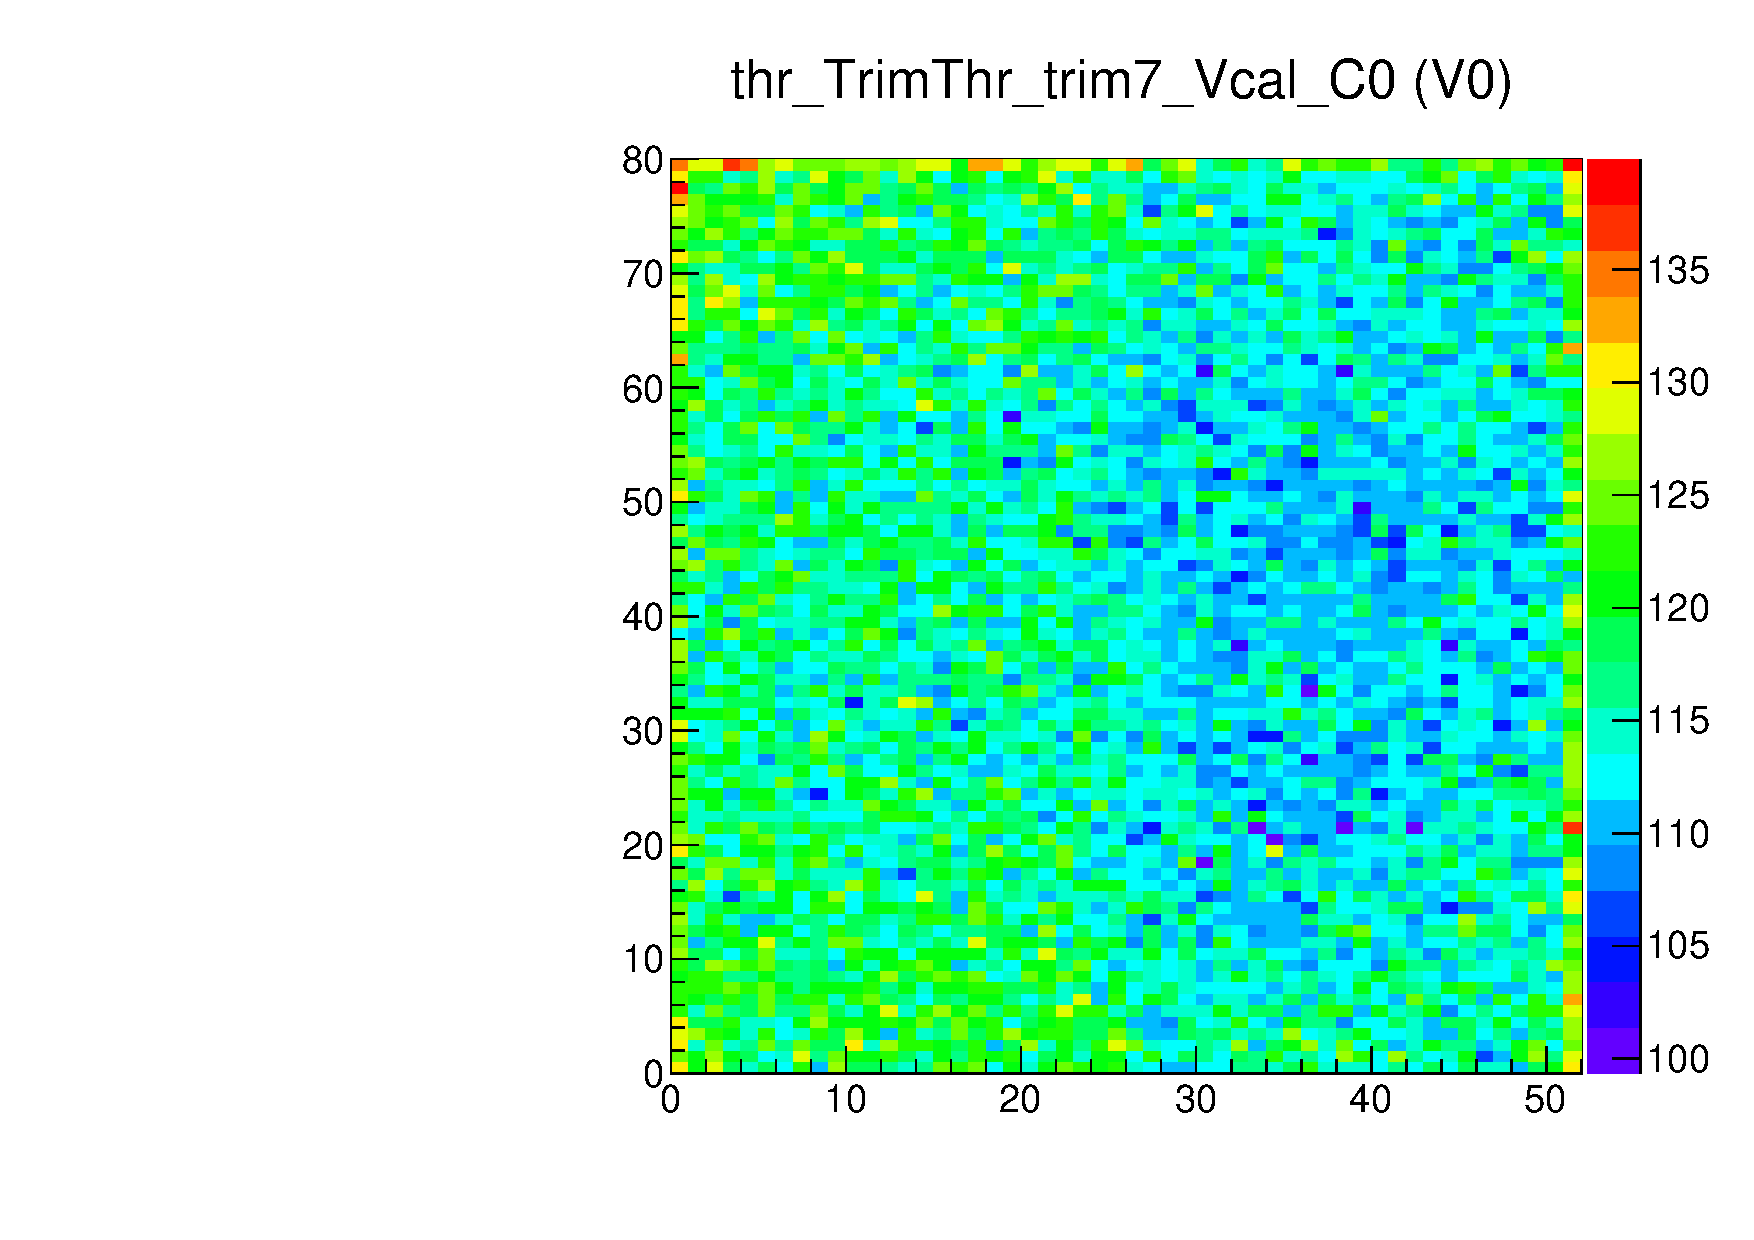
\includegraphics[width=1.0\textwidth]{figures/trim_thr_TrimThr_trim7_Vcal.pdf}
  \caption{}
  \label{fig:trim_thr_TrimThr_trim7_Vcal}
\end{minipage}
\end{figure}


% from trim bits test: difference in threshold wrt trimbits = 15

\begin{figure}[!Hp]
\centering
\begin{minipage}{0.45\textwidth}
  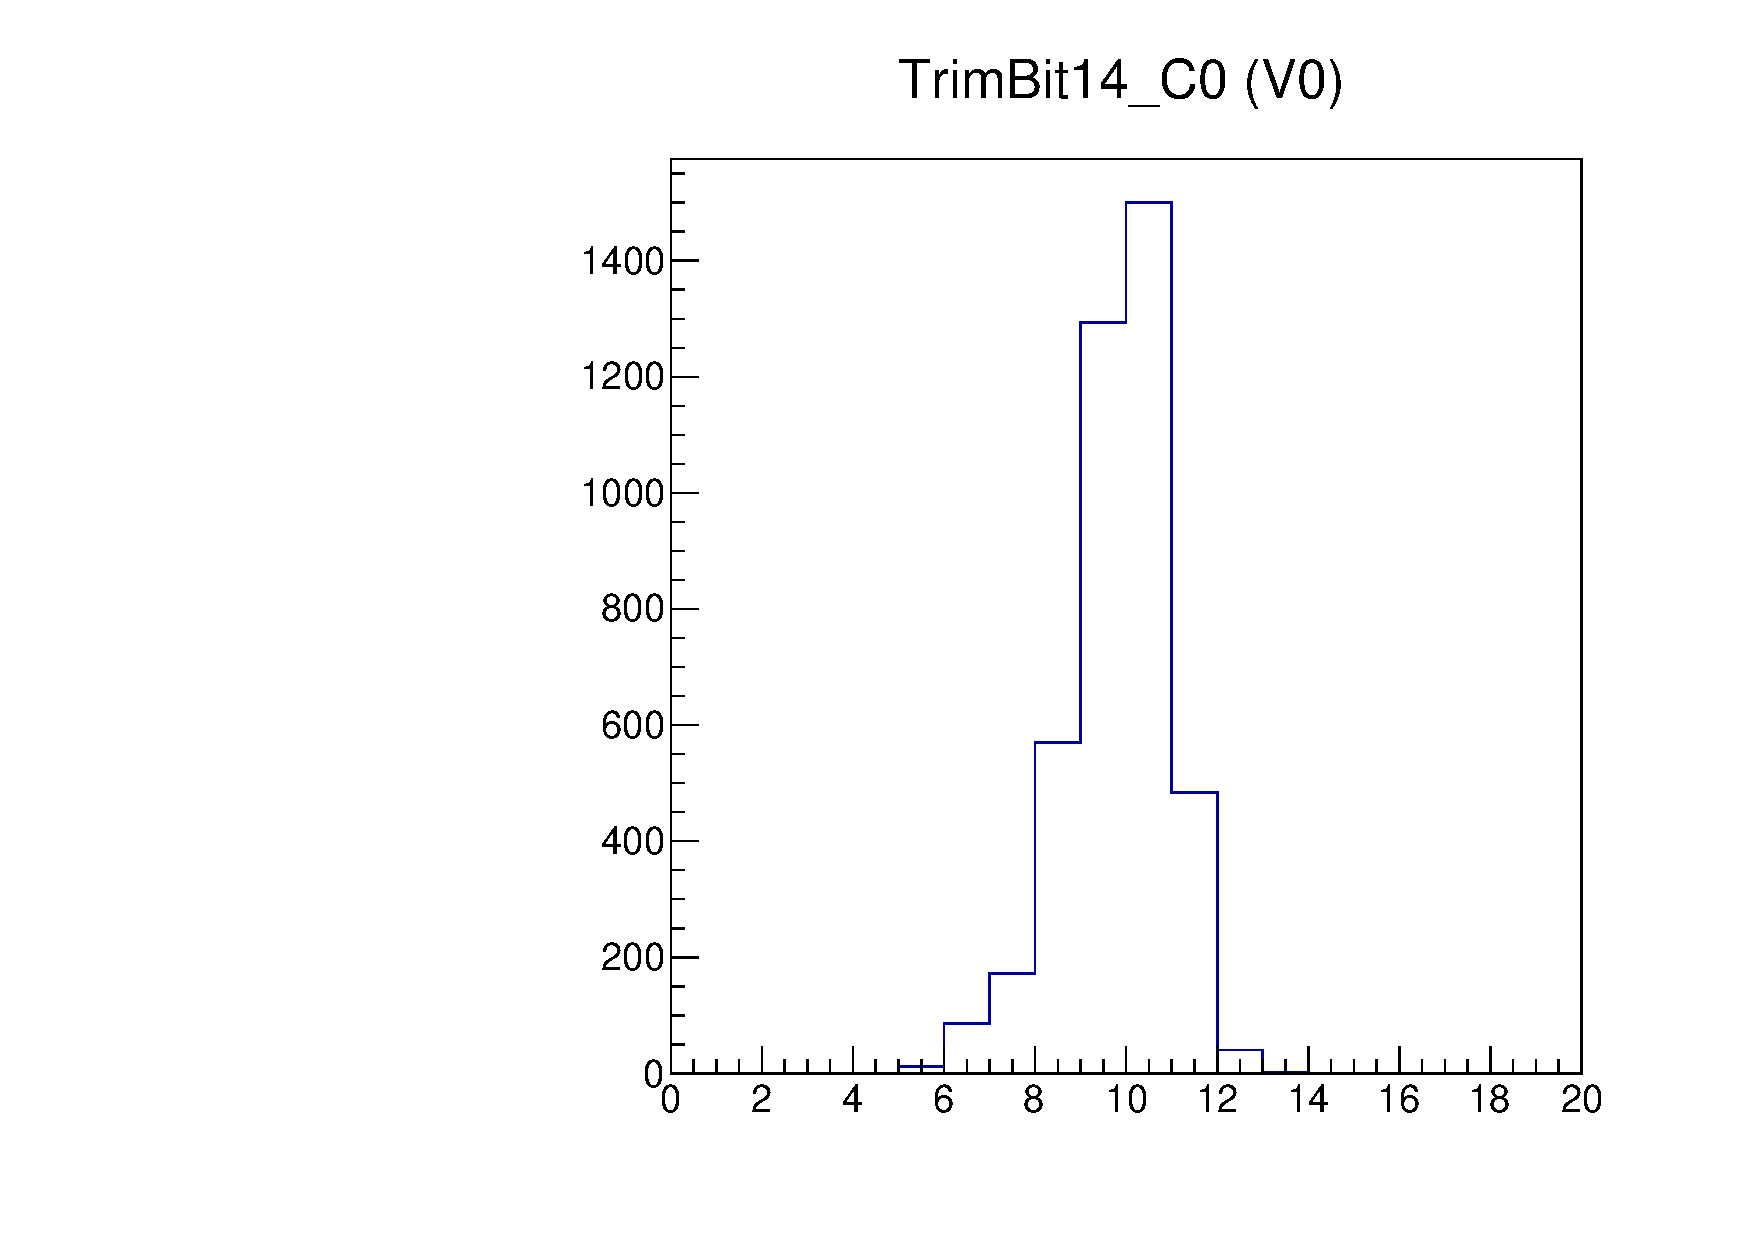
\includegraphics[width=1.0\textwidth]{figures/trim_TrimBit14.pdf}
  \caption{}
  \label{fig:trim_TrimBit14}
\end{minipage}
\hspace{0.3cm}
\begin{minipage}{0.45\textwidth}
  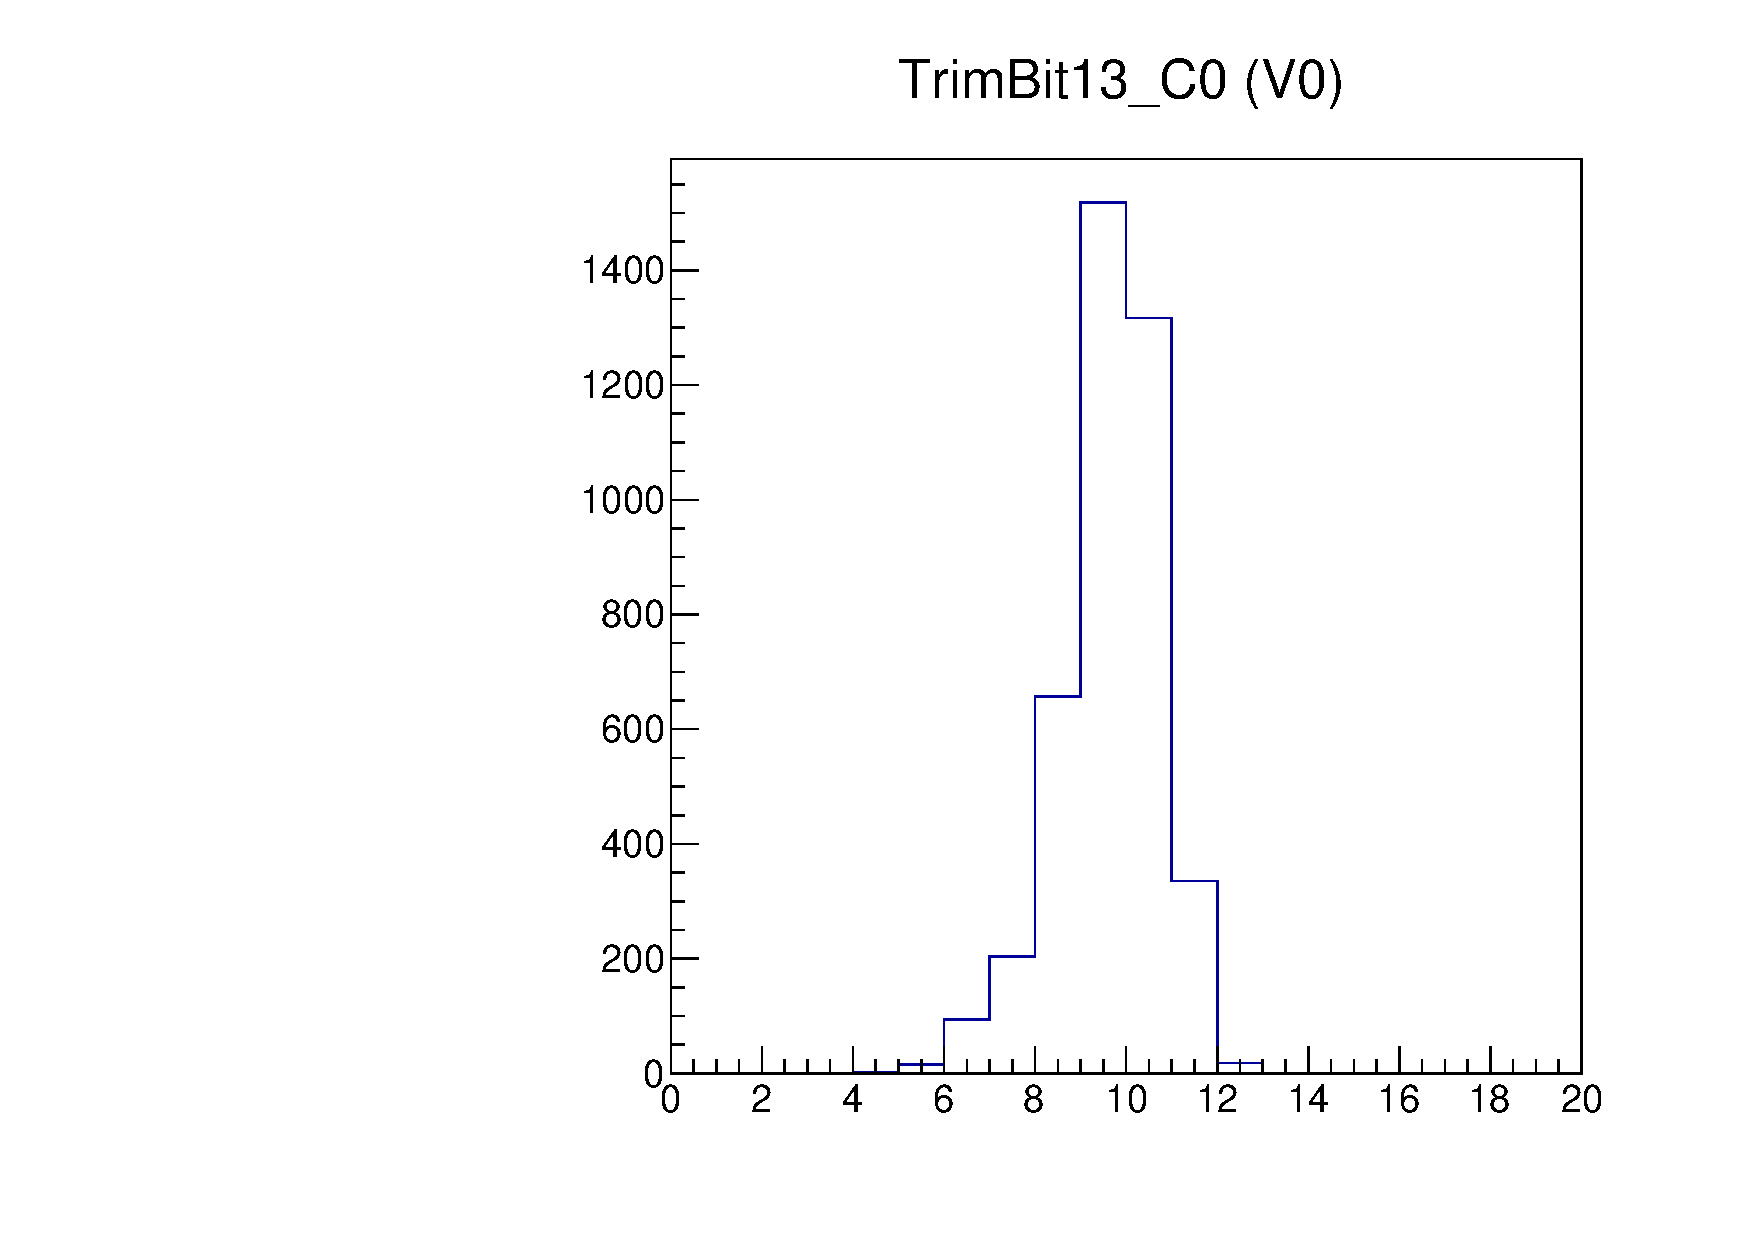
\includegraphics[width=1.0\textwidth]{figures/trim_TrimBit13.pdf}
  \caption{}
  \label{fig:trim_TrimBit13}
\end{minipage}
\end{figure}

\begin{figure}[!Hp]
\centering
\begin{minipage}{0.45\textwidth}
  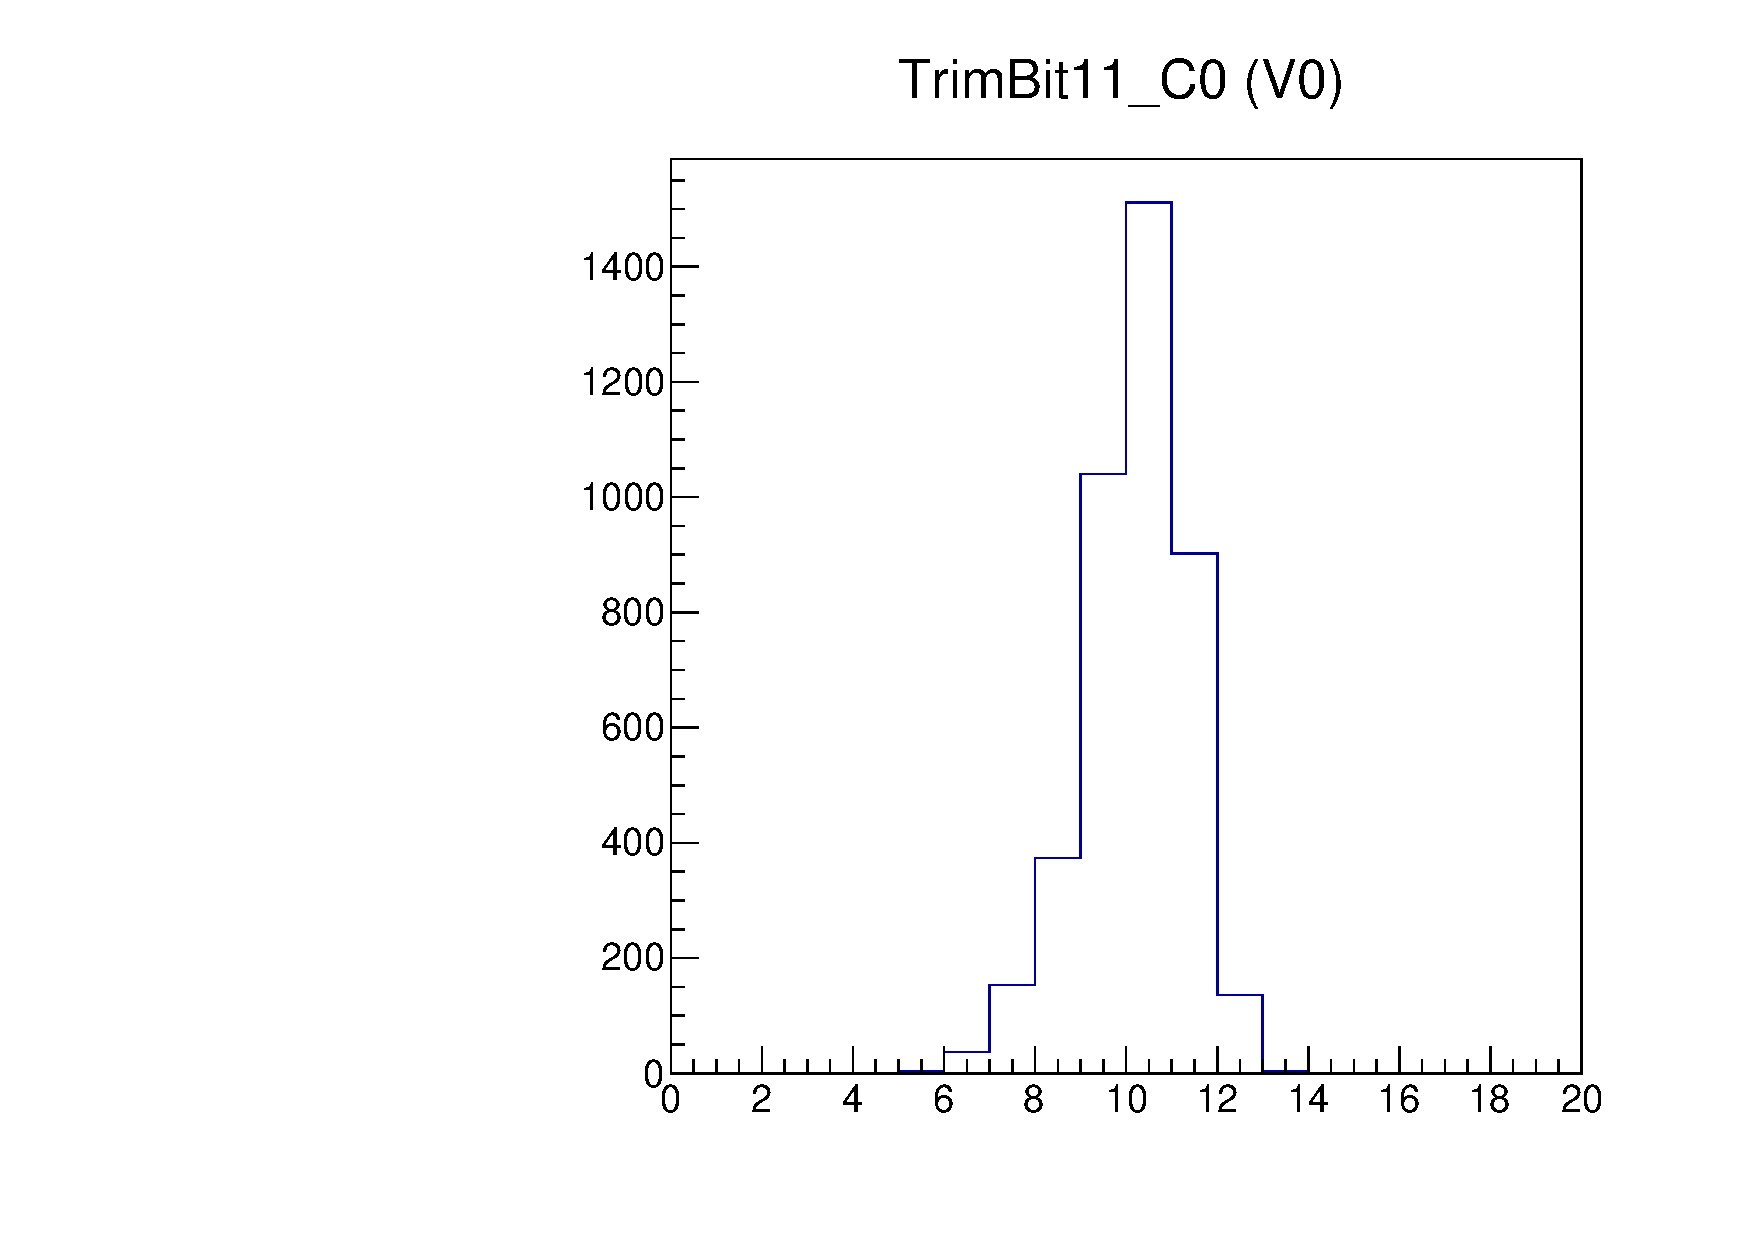
\includegraphics[width=1.0\textwidth]{figures/trim_TrimBit11.pdf}
  \caption{}
  \label{fig:trim_TrimBit11}
\end{minipage}
\hspace{0.3cm}
\begin{minipage}{0.45\textwidth}
  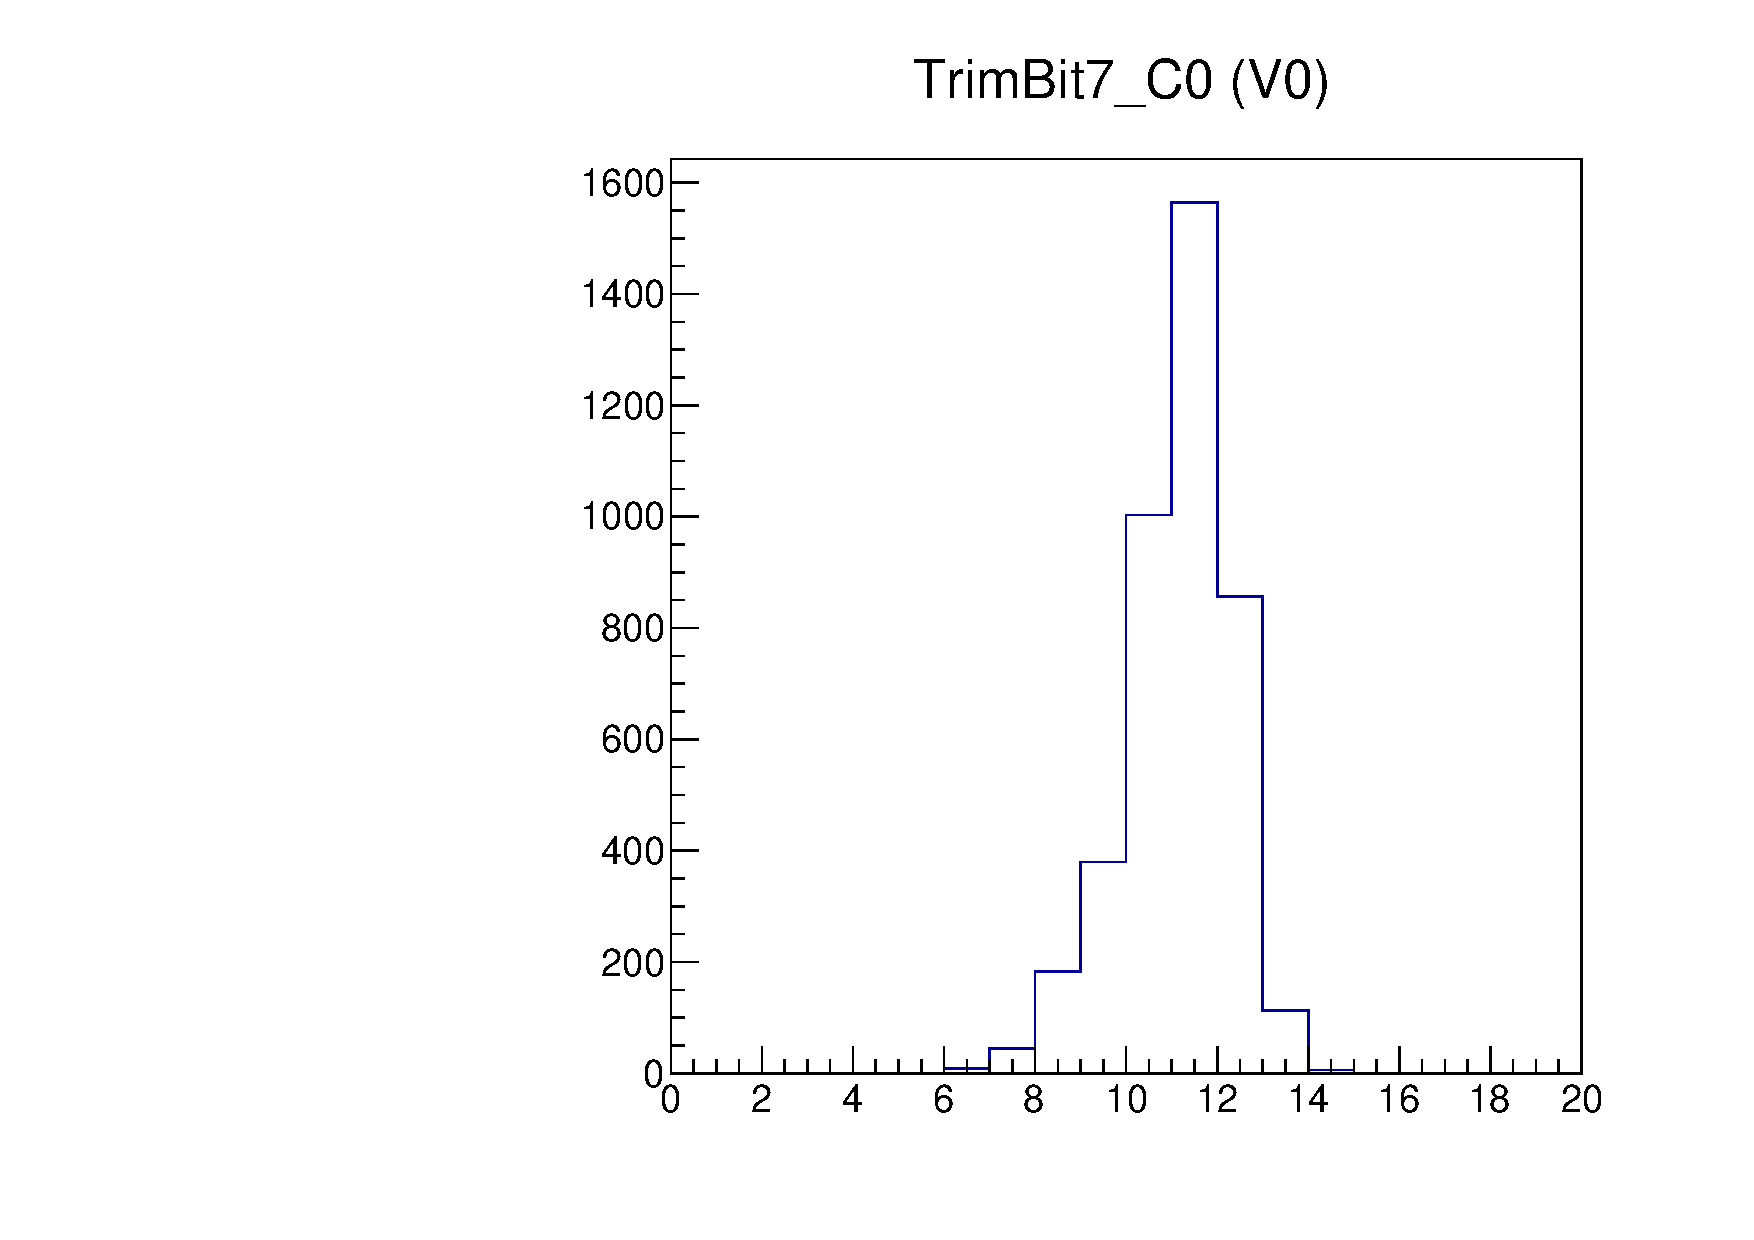
\includegraphics[width=1.0\textwidth]{figures/trim_TrimBit7.pdf}
  \caption{}
  \label{fig:trim_TrimBit7}
\end{minipage}
\end{figure}
